\documentclass{article}

\usepackage{arxiv}

\usepackage[utf8]{inputenc} % allow utf-8 input
\usepackage[T1]{fontenc}    % use 8-bit T1 fonts
\usepackage{lmodern}        % https://github.com/rstudio/rticles/issues/343
\usepackage{hyperref}       % hyperlinks
\usepackage{url}            % simple URL typesetting
\usepackage{booktabs}       % professional-quality tables
\usepackage{amsfonts}       % blackboard math symbols
\usepackage{nicefrac}       % compact symbols for 1/2, etc.
\usepackage{microtype}      % microtypography
\usepackage{graphicx}

\title{Unveiling Color Dynamics in Andy Warhol's ``Shot Marilyns'': A
Study on Visual Variations and Perception}

\author{
    Erick S. Arenas V
   \\
    Department of Statistics \\
    University of California, Davis \\
  Davis, CA 95616 \\
  \texttt{\href{mailto:esarenas@ucdavis.edu}{\nolinkurl{esarenas@ucdavis.edu}}} \\
   \And
    Weilin Cheng
   \\
    Department of Statistics \\
    University of California, Davis \\
  Davis, CA 95616 \\
  \texttt{\href{mailto:wncheng@ucdavis.edu}{\nolinkurl{wncheng@ucdavis.edu}}} \\
   \And
    Hengyuan Liu
   \\
    Department of Statistics \\
    University of California, Los Angeles \\
  Los Angeles, CA 90095 \\
  \texttt{\href{mailto:hengyuanliu@g.ucla.edu}{\nolinkurl{hengyuanliu@g.ucla.edu}}} \\
   \And
    Xinhui Luo
   \\
    Department of Statistics \\
    Tufts University \\
  Boston, MA 02155 \\
  \texttt{\href{mailto:xinhui.luo@tufts.edu}{\nolinkurl{xinhui.luo@tufts.edu}}} \\
   \And
    Kathy Mo
   \\
    Department of Statistics \\
    University of California, Los Angeles \\
  Los Angeles, CA 90095 \\
  \texttt{\href{mailto:kathymo24@g.ucla.edu}{\nolinkurl{kathymo24@g.ucla.edu}}} \\
   \And
    Li Yuan
   \\
    Department of Statistics \\
    University of Michigan, Ann Arbor \\
  Ann Arbor, MI 48109 \\
  \texttt{\href{mailto:leeyuan@umich.edu}{\nolinkurl{leeyuan@umich.edu}}} \\
  }


% tightlist command for lists without linebreak
\providecommand{\tightlist}{%
  \setlength{\itemsep}{0pt}\setlength{\parskip}{0pt}}



\usepackage{amsmath}
\usepackage{graphicx}
\usepackage{subcaption}
\begin{document}
\maketitle


\begin{abstract}
This study delves into the comparative analysis of five distinct
versions of Andy Warhol's ``Shot Marilyns,'' focusing on the intricacies
of their color composition and distribution. Employing a range of
analytical methods, including relative conditional entropy, this
research investigates the unique color distributions and interrelations
present in each artwork. Through the clustering of the artworks and the
meticulous examination of specified regions of interest (ROIs)---namely,
the backgrounds, hair, eyeshadow, and faces---we have unearthed profound
insights into the constructional variances and similarities among the
images. Our findings reveal that the presupposed uniformity in the
coloration of certain elements stands contradicted, thereby underscoring
the complexity and illusionary nature of color perception in visual art.
\end{abstract}

\keywords{
    shot marilyns
   \and
    marilyn monroe
   \and
    andy warhol
   \and
    region of interest
   \and
    python
  }

\hypertarget{introduction}{%
\section{Introduction}\label{introduction}}

``Shot Marilyns,'' an illustrious artwork by the American artist Andy
Warhol, stands as a testament to his exploration of celebrity culture
and the commodification of images. Created in 1964, this series features
multiple depictions of Marilyn Monroe, crafted in the wake of her
untimely demise, thereby immortalizing her status as a cultural icon.
Warhol's fascination with fame, consumerism, and the media's influence
on societal perceptions is evident in his innovative use of silkscreen
printing. This technique, adopted in August 1962, facilitated a
production-line approach in art-making, enabling Warhol to replicate
images with minor variations. The ``Shot Marilyns'' series, inspired by
Monroe's death in the same year, utilized this method to produce
screenprints of her image, employing photo stencils and a palette of
vibrant inks to transfer her likeness onto canvas. This body of work
underscores Warhol's endeavor to dissect Monroe's persona through
repetitive imagery, each variation rendered in distinct colors and
compositions, allowing for diverse visual interpretations.

The series' repetitive nature serves as a critique of the pervasive
commodification of celebrities, transforming them into ubiquitous
symbols within popular culture. Warhol's strategic use of bright,
contrasting colors aims to encapsulate Monroe's dynamic celebrity
essence, with the vivid hues underscoring her societal allure and
influence. This study seeks to analyze the pixel color distribution in
RGB space across the five ``Shot Marilyns'' images, examining the
interplay between primary colors through relative conditional entropy.
Such an analysis aims to reveal the underlying emotional and symbolic
connotations Warhol might have intended, with color distributions
potentially reflecting varied moods and themes.

In 1964, an intriguing incident further contributed to the series' lore
when Dorothy Podber, a performance artist, mistakenly received
permission from Warhol to ``shoot'' the Marilyns, leading to an act of
literal gunfire that damaged four of the five canvases. This event
birthed the ``Shot Marilyns,'' adding a layer of physical and conceptual
depth to the artwork. Part of our project involves digitally restoring
the ``Blue Marilyn,'' focusing on the gunshot damage, by analyzing and
replicating the surrounding area's color distribution.

This paper is intended for publication in the Journal on Computing and
Cultural Heritage and aims to shed light on the technological
intersections of art restoration and analysis, using Warhol's ``Shot
Marilyns'' as a pivotal study case.

\begin{figure}[ht]
  \centering
  \begin{subfigure}{0.3\textwidth}
    \centering
    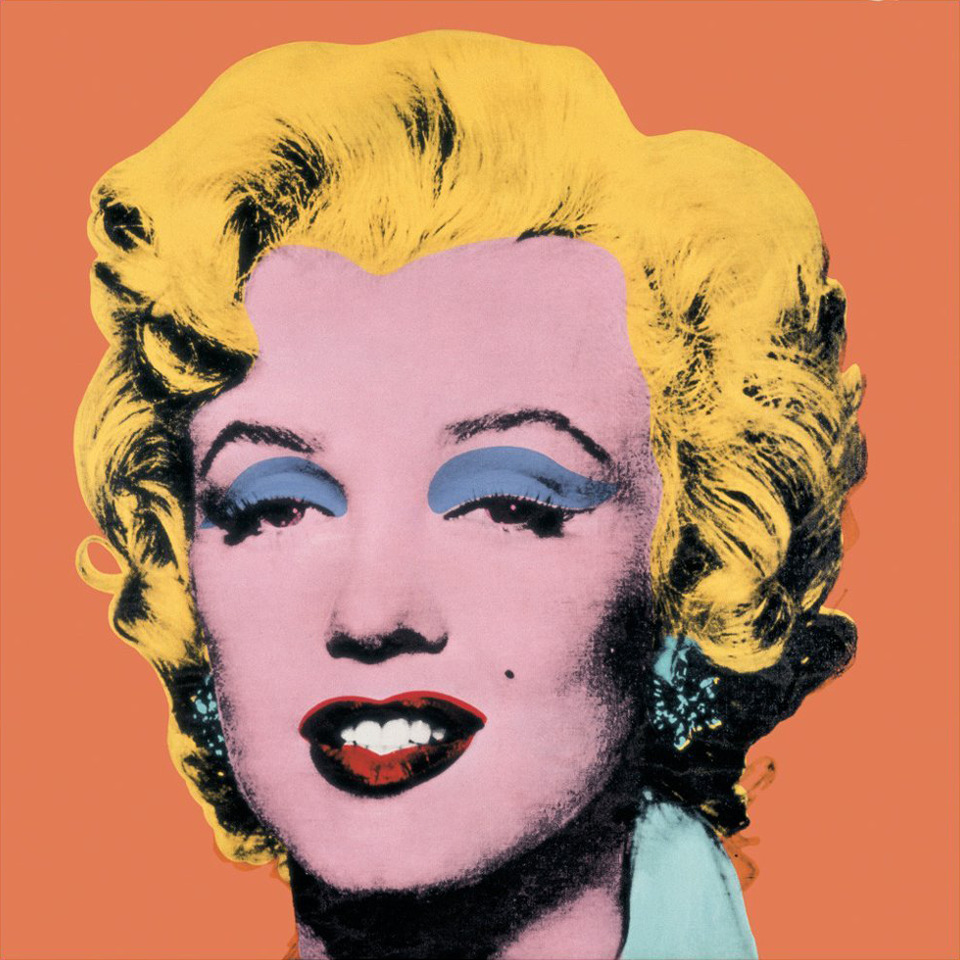
\includegraphics[width=125px]{main_files/figure-latex/1_1_orange_marilyn.jpg}
    \caption{Figure 1.1: Orange Marilyn}
    \label{fig:1_1_orange_marilyn}
  \end{subfigure}
  \hfill
  \begin{subfigure}{0.3\textwidth}
    \centering
    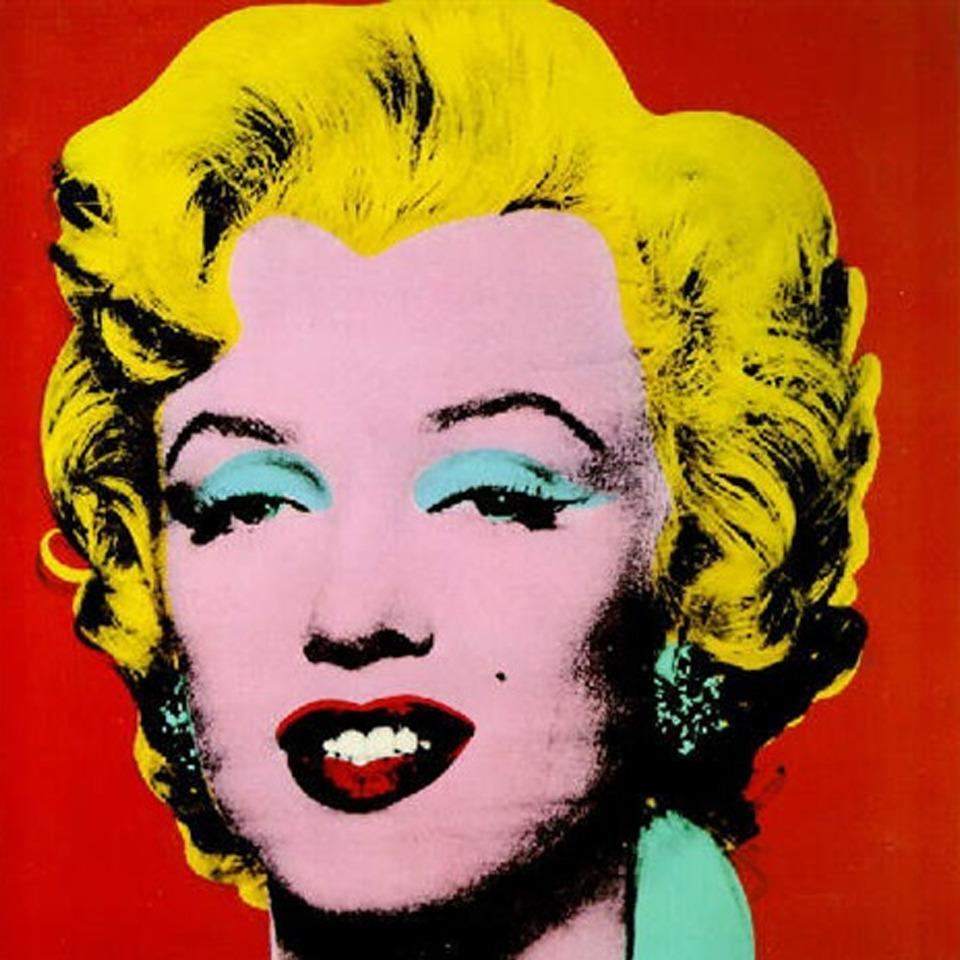
\includegraphics[width=125px]{main_files/figure-latex/1_2_red_marilyn.jpg}
    \caption{Figure 1.2: Red Marilyn}
    \label{fig:1_2_red_marilyn}
  \end{subfigure}
  \hfill
  \begin{subfigure}{0.3\textwidth}
    \centering
    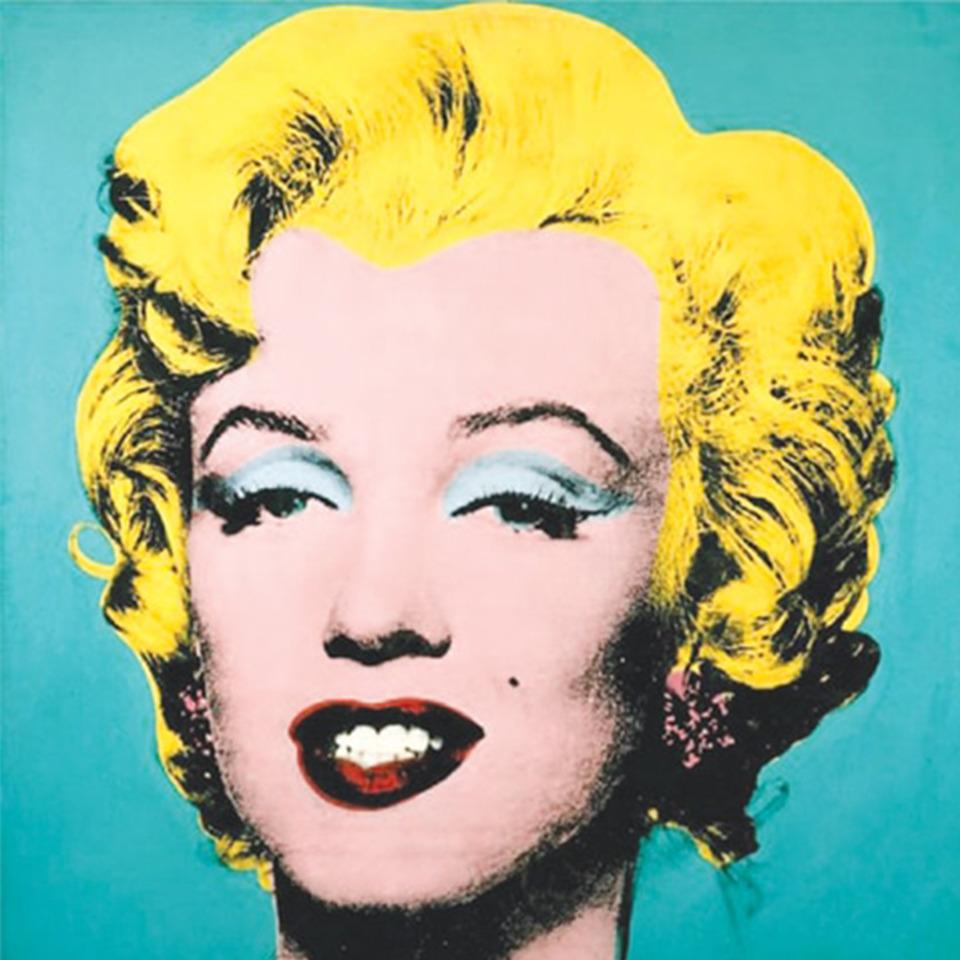
\includegraphics[width=125px]{main_files/figure-latex/1_3_turq_marilyn.jpg}
    \caption{Figure 1.3: Turquoise Marilyn}
    \label{fig:1_3_turq_marilyn}
  \end{subfigure}

  \vspace{1em} % Add some vertical space between rows

  \begin{minipage}{0.6\textwidth}
    \centering
    \begin{subfigure}{0.45\textwidth}
      \centering
      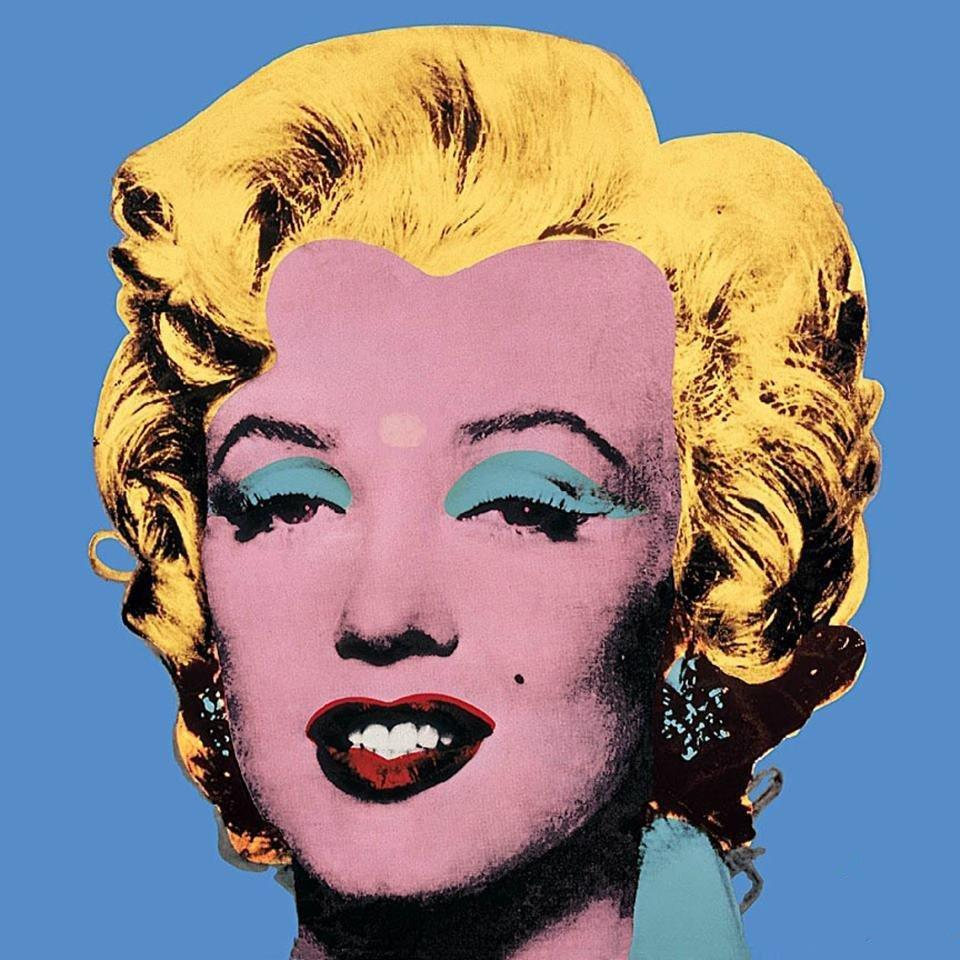
\includegraphics[width=125px]{main_files/figure-latex/1_4_blue_marilyn.jpg}
      \caption{Figure 1.4: Blue Marilyn}
      \label{fig:1_4_blue_marilyn}
    \end{subfigure}
    \hfill
    \begin{subfigure}{0.45\textwidth}
      \centering
      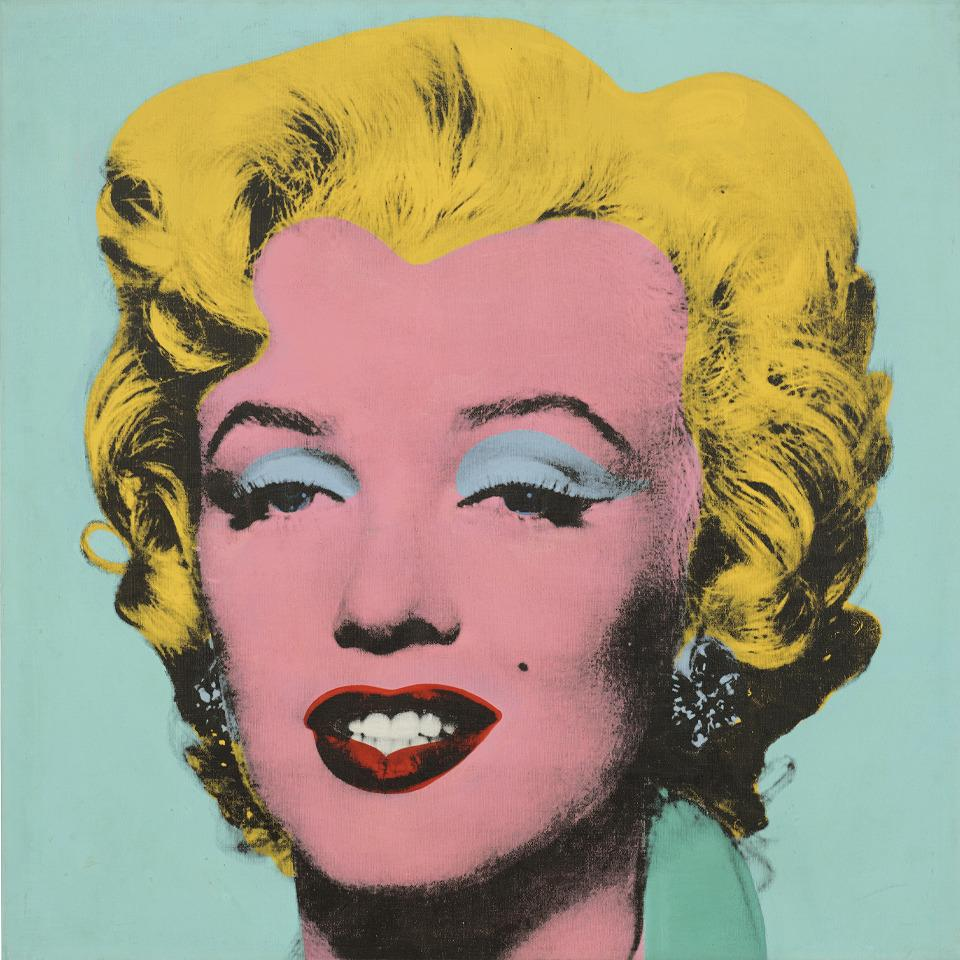
\includegraphics[width=125px]{main_files/figure-latex/1_5_eggblue_marilyn.jpg}
      \caption{Figure 1.5: Eggblue Marilyn}
      \label{fig:1_5_eggblue_marilyn}
    \end{subfigure}
  \end{minipage}

  \caption{Different color variations of Marilyn Monroe}
  \label{fig:marilyn_variations}
\end{figure}

\hypertarget{methods}{%
\section{Methods}\label{methods}}

An image comprises pixels, with each pixel containing three color
components: Red (R), Green (G), and Blue (B), denoted as (R, G, B)
respectively. These components define the intensity of the respective
colors, with each component represented by an integer value within the
range of {[}0, 255{]} in the RGB color space. Therefore, each color
component is a discrete variable capable of assuming 256 distinct
values. In the equations below, \(Y=y\) or \(X=x\) can be selected from
any of the three color components, R, G, or B.

\hypertarget{entropy-calculation}{%
\subsection{Entropy Calculation}\label{entropy-calculation}}

The probability of a specific color component, \(P(Y=y)\), is determined
by dividing the number of pixels with color coordinates corresponding to
that component by the total number of color components in the entire
image. The following equations illustrate the calculation of entropy,
conditional entropy, and relative conditional entropy

The entropy of a color component \(Y\) is defined as:

\begin{equation}
    H(Y) = - \sum_{y=0}^{255} P(Y = y) \cdot \log(P(Y = y))
\end{equation}

The conditional entropy of \(Y\) given \(X\) is given by:

\begin{equation}
    H(Y|X) = \sum_{x=0}^{255} P(X = x) \cdot H(Y|X = x) = - \sum_{x=0}^{255} \sum_{y=0}^{255} P(X = x, Y = y) \log_2 \left(\frac{P(X = x, Y = y)}{P(X = x)}\right)
\end{equation}

The relative conditional entropy is calculated using the following
formula:

\begin{equation}
    HR(X|Y) = \frac{H(X|Y)}{H(X)}
\end{equation}

\hypertarget{k-means-clustering-analysis}{%
\subsection{K-Means Clustering
Analysis}\label{k-means-clustering-analysis}}

XXXXXXXXX\ldots.

\hypertarget{data-description}{%
\section{Data Description}\label{data-description}}

Our study utilized a dataset comprising five images, each retrieved via
URL links provided by ``The Interior Review'' website {[}1{]}. The
images, titled Orange Marilyn, Red Marilyn, Turquoise Marilyn, Blue
Marilyn, and Eggblue Marilyn, are digitally encoded in the RGB color
model. This model synthesizes a spectrum of colors through the additive
mixing of Red, Green, and Blue light. The intensity of each primary
color is quantized into discrete levels, ranging from 0 to 255, offering
a finite palette within this cubic color space. The dimensions of each
image are 960 by 960 pixels, totaling 921,600 unique data points per
image, each specified by a distinct location and its chromatic
composition.

\hypertarget{data-exploration-and-visualization-analysis}{%
\section{Data Exploration and Visualization
Analysis}\label{data-exploration-and-visualization-analysis}}

\begin{figure}[ht]
  \centering
  \begin{subfigure}{0.3\textwidth}
    \centering
    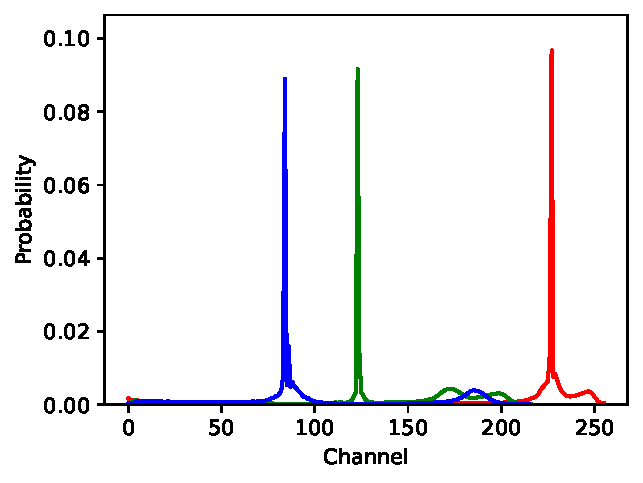
\includegraphics[width=125px]{main_files/figure-latex/2_1_orange_marilyn_dist.pdf}
    \caption{Figure 1.1: Orange Marilyn}
    \label{fig:1_1_orange_marilyn}
  \end{subfigure}
  \hfill
  \begin{subfigure}{0.3\textwidth}
    \centering
    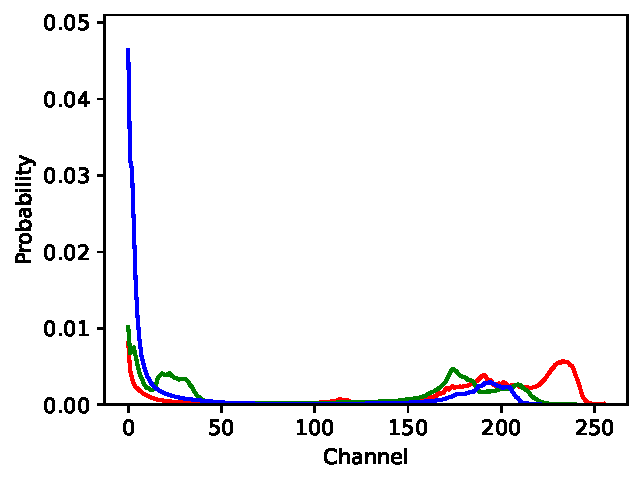
\includegraphics[width=125px]{main_files/figure-latex/2_2_red_marilyn_dist.pdf}
    \caption{Figure 1.2: Red Marilyn}
    \label{fig:1_2_red_marilyn}
  \end{subfigure}
  \hfill
  \begin{subfigure}{0.3\textwidth}
    \centering
    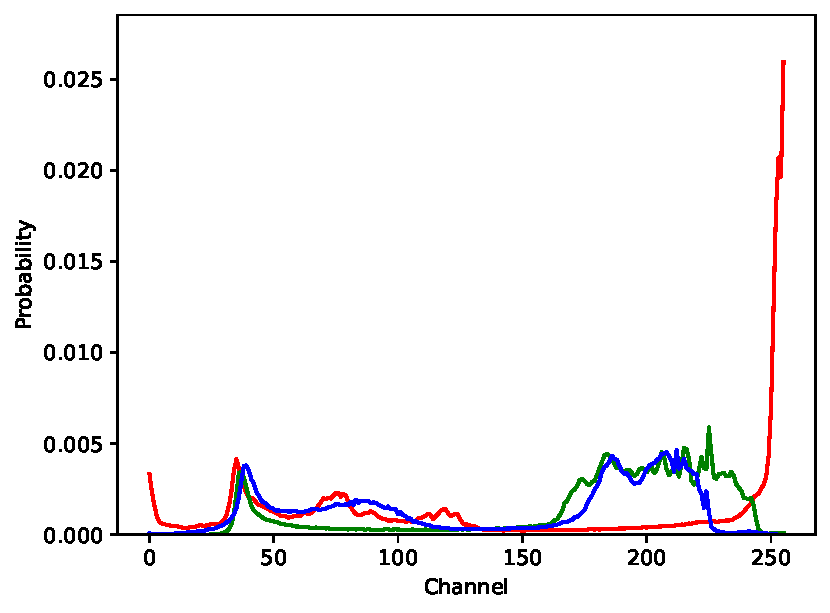
\includegraphics[width=125px]{main_files/figure-latex/2_3_turq_marilyn_dist.pdf}
    \caption{Figure 1.3: Turquoise Marilyn}
    \label{fig:1_3_turq_marilyn}
  \end{subfigure}

  \vspace{1em} % Add some vertical space between rows

  \begin{minipage}{0.6\textwidth}
    \centering
    \begin{subfigure}{0.45\textwidth}
      \centering
      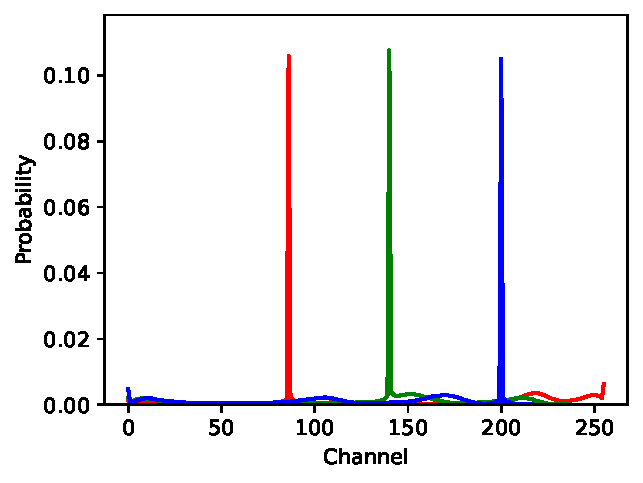
\includegraphics[width=125px]{main_files/figure-latex/2_4_blue_marilyn_dist.pdf}
      \caption{Figure 1.4: Blue Marilyn}
      \label{fig:1_4_blue_marilyn}
    \end{subfigure}
    \hfill
    \begin{subfigure}{0.45\textwidth}
      \centering
      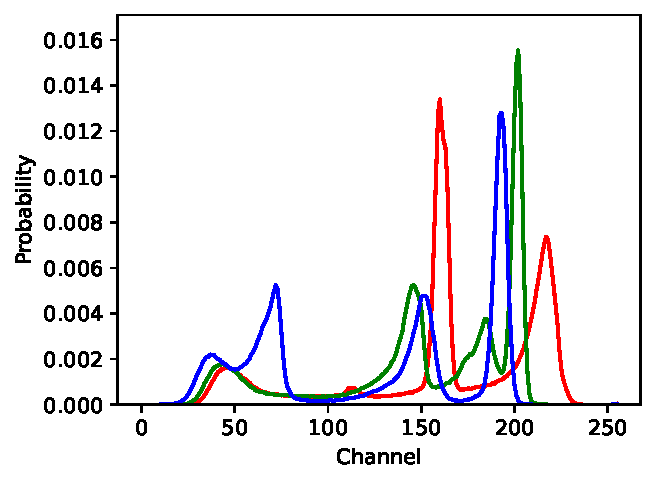
\includegraphics[width=125px]{main_files/figure-latex/2_5_eggblue_marilyn_dist.pdf}
      \caption{Figure 1.5: Eggblue Marilyn}
      \label{fig:1_5_eggblue_marilyn}
    \end{subfigure}
  \end{minipage}

  \caption{Different color variations of Marilyn Monroe}
  \label{fig:marilyn_variations}
\end{figure}

Our initial analytical procedure involved scrutinizing the RGB channels
of the images and assessing their distribution profiles. Figure 3
delineates the variation in the red, green, and blue distributions
across the five images. Notably, images (A) and (D) display pronounced
disparities when contrasted with the others. For instance, in the (A)
Orange Marilyn image, the blue channel's most significant probability
density is localized within the {[}50, 100{]} interval, reaching an
estimated 27\%. The green channel's peak probability lies between
{[}120, 130{]}, at around 28\%. Similarly, a notable concentration for
blue is observed in the {[}220, 240{]} range with a likelihood of
approximately 29\%.

Intriguingly, image (D) mirrors the (A) Orange Marilyn in terms of green
channel probabilities, predominantly in the {[}120, 130{]} range.
However, it diverges markedly in the red and blue spectra. Image (D)
features a red channel probability apex in the {[}70, 80{]} interval,
representing a 32\% likelihood, while its blue channel's highest
probability is within the {[}190, 210{]} range, also accounting for a
32\% probability. The divergence in the red and blue channel
distributions between images (D) and (A) accentuates their unique
attributes in the collective color distribution.

\begin{figure}[ht]
  \centering
  \begin{subfigure}{0.3\textwidth}
    \centering
    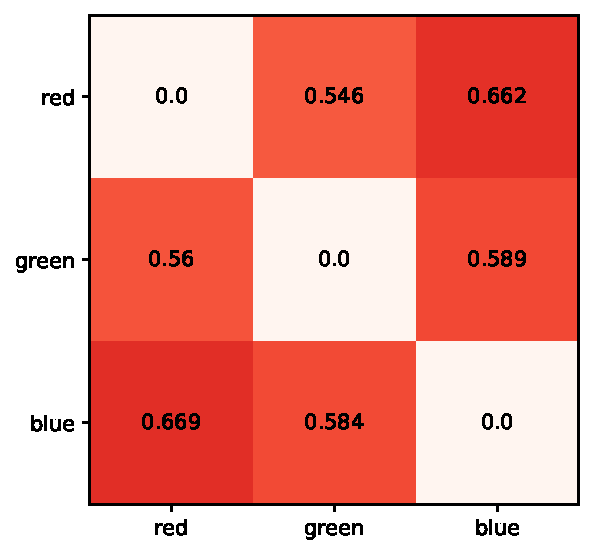
\includegraphics[width=125px]{main_files/figure-latex/3_1_orange_marilyn_entropy.pdf}
    \caption{Figure 1.1: Orange Marilyn}
    \label{fig:1_1_orange_marilyn}
  \end{subfigure}
  \hfill
  \begin{subfigure}{0.3\textwidth}
    \centering
    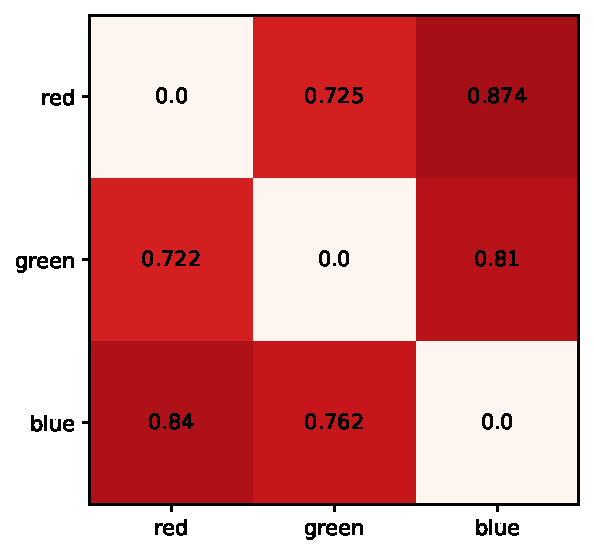
\includegraphics[width=125px]{main_files/figure-latex/3_2_red_marilyn_entropy.pdf}
    \caption{Figure 1.2: Red Marilyn}
    \label{fig:1_2_red_marilyn}
  \end{subfigure}
  \hfill
  \begin{subfigure}{0.3\textwidth}
    \centering
    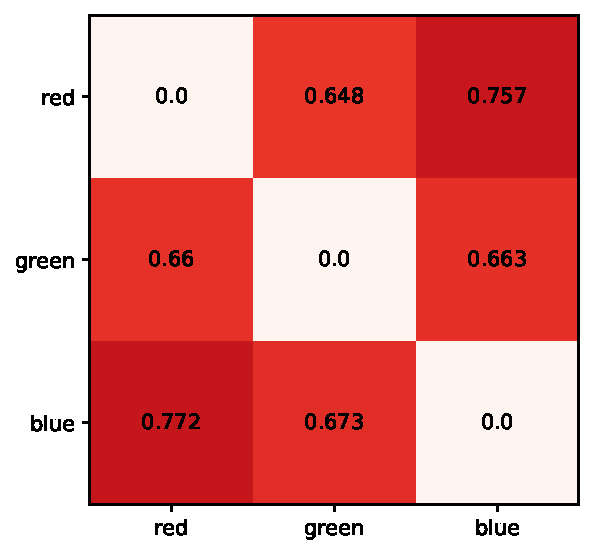
\includegraphics[width=125px]{main_files/figure-latex/3_3_turq_marilyn_entropy.pdf}
    \caption{Figure 1.3: Turquoise Marilyn}
    \label{fig:1_3_turq_marilyn}
  \end{subfigure}

  \vspace{1em} % Add some vertical space between rows

  \begin{minipage}{0.6\textwidth}
    \centering
    \begin{subfigure}{0.45\textwidth}
      \centering
      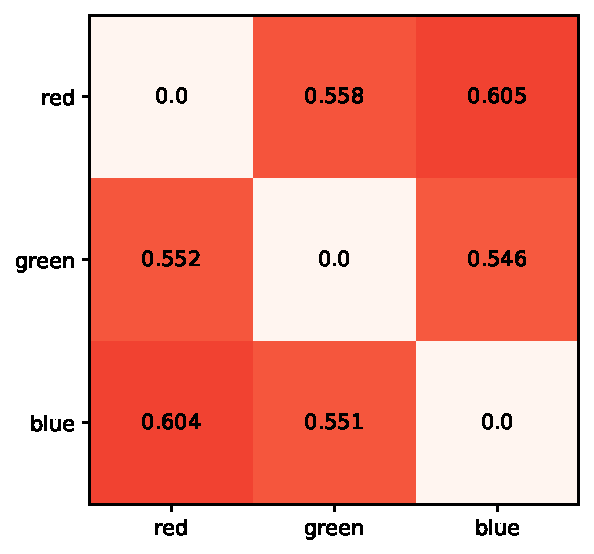
\includegraphics[width=125px]{main_files/figure-latex/3_4_blue_marilyn_entropy.pdf}
      \caption{Figure 1.4: Blue Marilyn}
      \label{fig:1_4_blue_marilyn}
    \end{subfigure}
    \hfill
    \begin{subfigure}{0.45\textwidth}
      \centering
      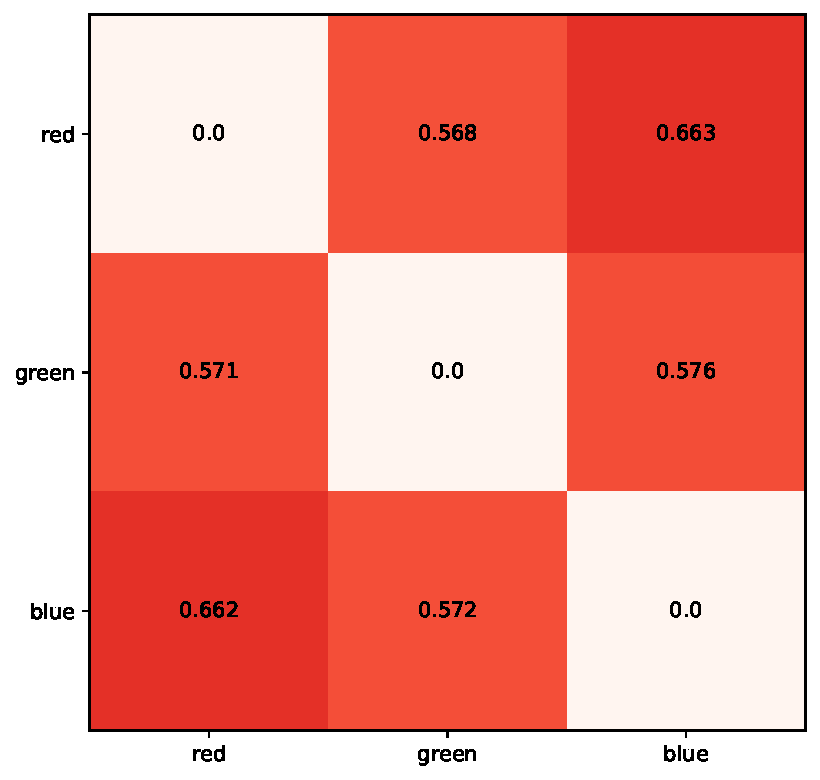
\includegraphics[width=125px]{main_files/figure-latex/3_5_eggblue_marilyn_entropy.pdf}
      \caption{Figure 1.5: Eggblue Marilyn}
      \label{fig:1_5_eggblue_marilyn}
    \end{subfigure}
  \end{minipage}

  \caption{Different color variations of Marilyn Monroe}
  \label{fig:marilyn_variations}
\end{figure}

\hypertarget{clustering-based-on-whole-images}{%
\section{Clustering based on Whole
Images}\label{clustering-based-on-whole-images}}

To analyze the distribution of RGB colors in a 2D space, we plotted each
color channel against the others for the entire image. Figures 5 to 9
display a series of scatter plots, with each dot representing a single
pixel. The top three scatter plots in each figure show the distribution
of pixel colors in the 2D RGB space, using combinations of Red, Green,
and Blue coordinates. The bottom three scatter plots use grayscale to
represent the intensity of each color component. In these grayscale
plots, lower intensity values appear as white, while higher intensity
values appear as black. Specifically, the leftmost panel illustrates the
relationship between red and green, with blue represented in grayscale.
The middle panel shows the interplay between red and blue, with green in
grayscale. The rightmost panel depicts the interaction between green and
blue, with red in grayscale.

\begin{figure}[ht]
  \centering
  \begin{subfigure}{0.45\textwidth}
    \centering
    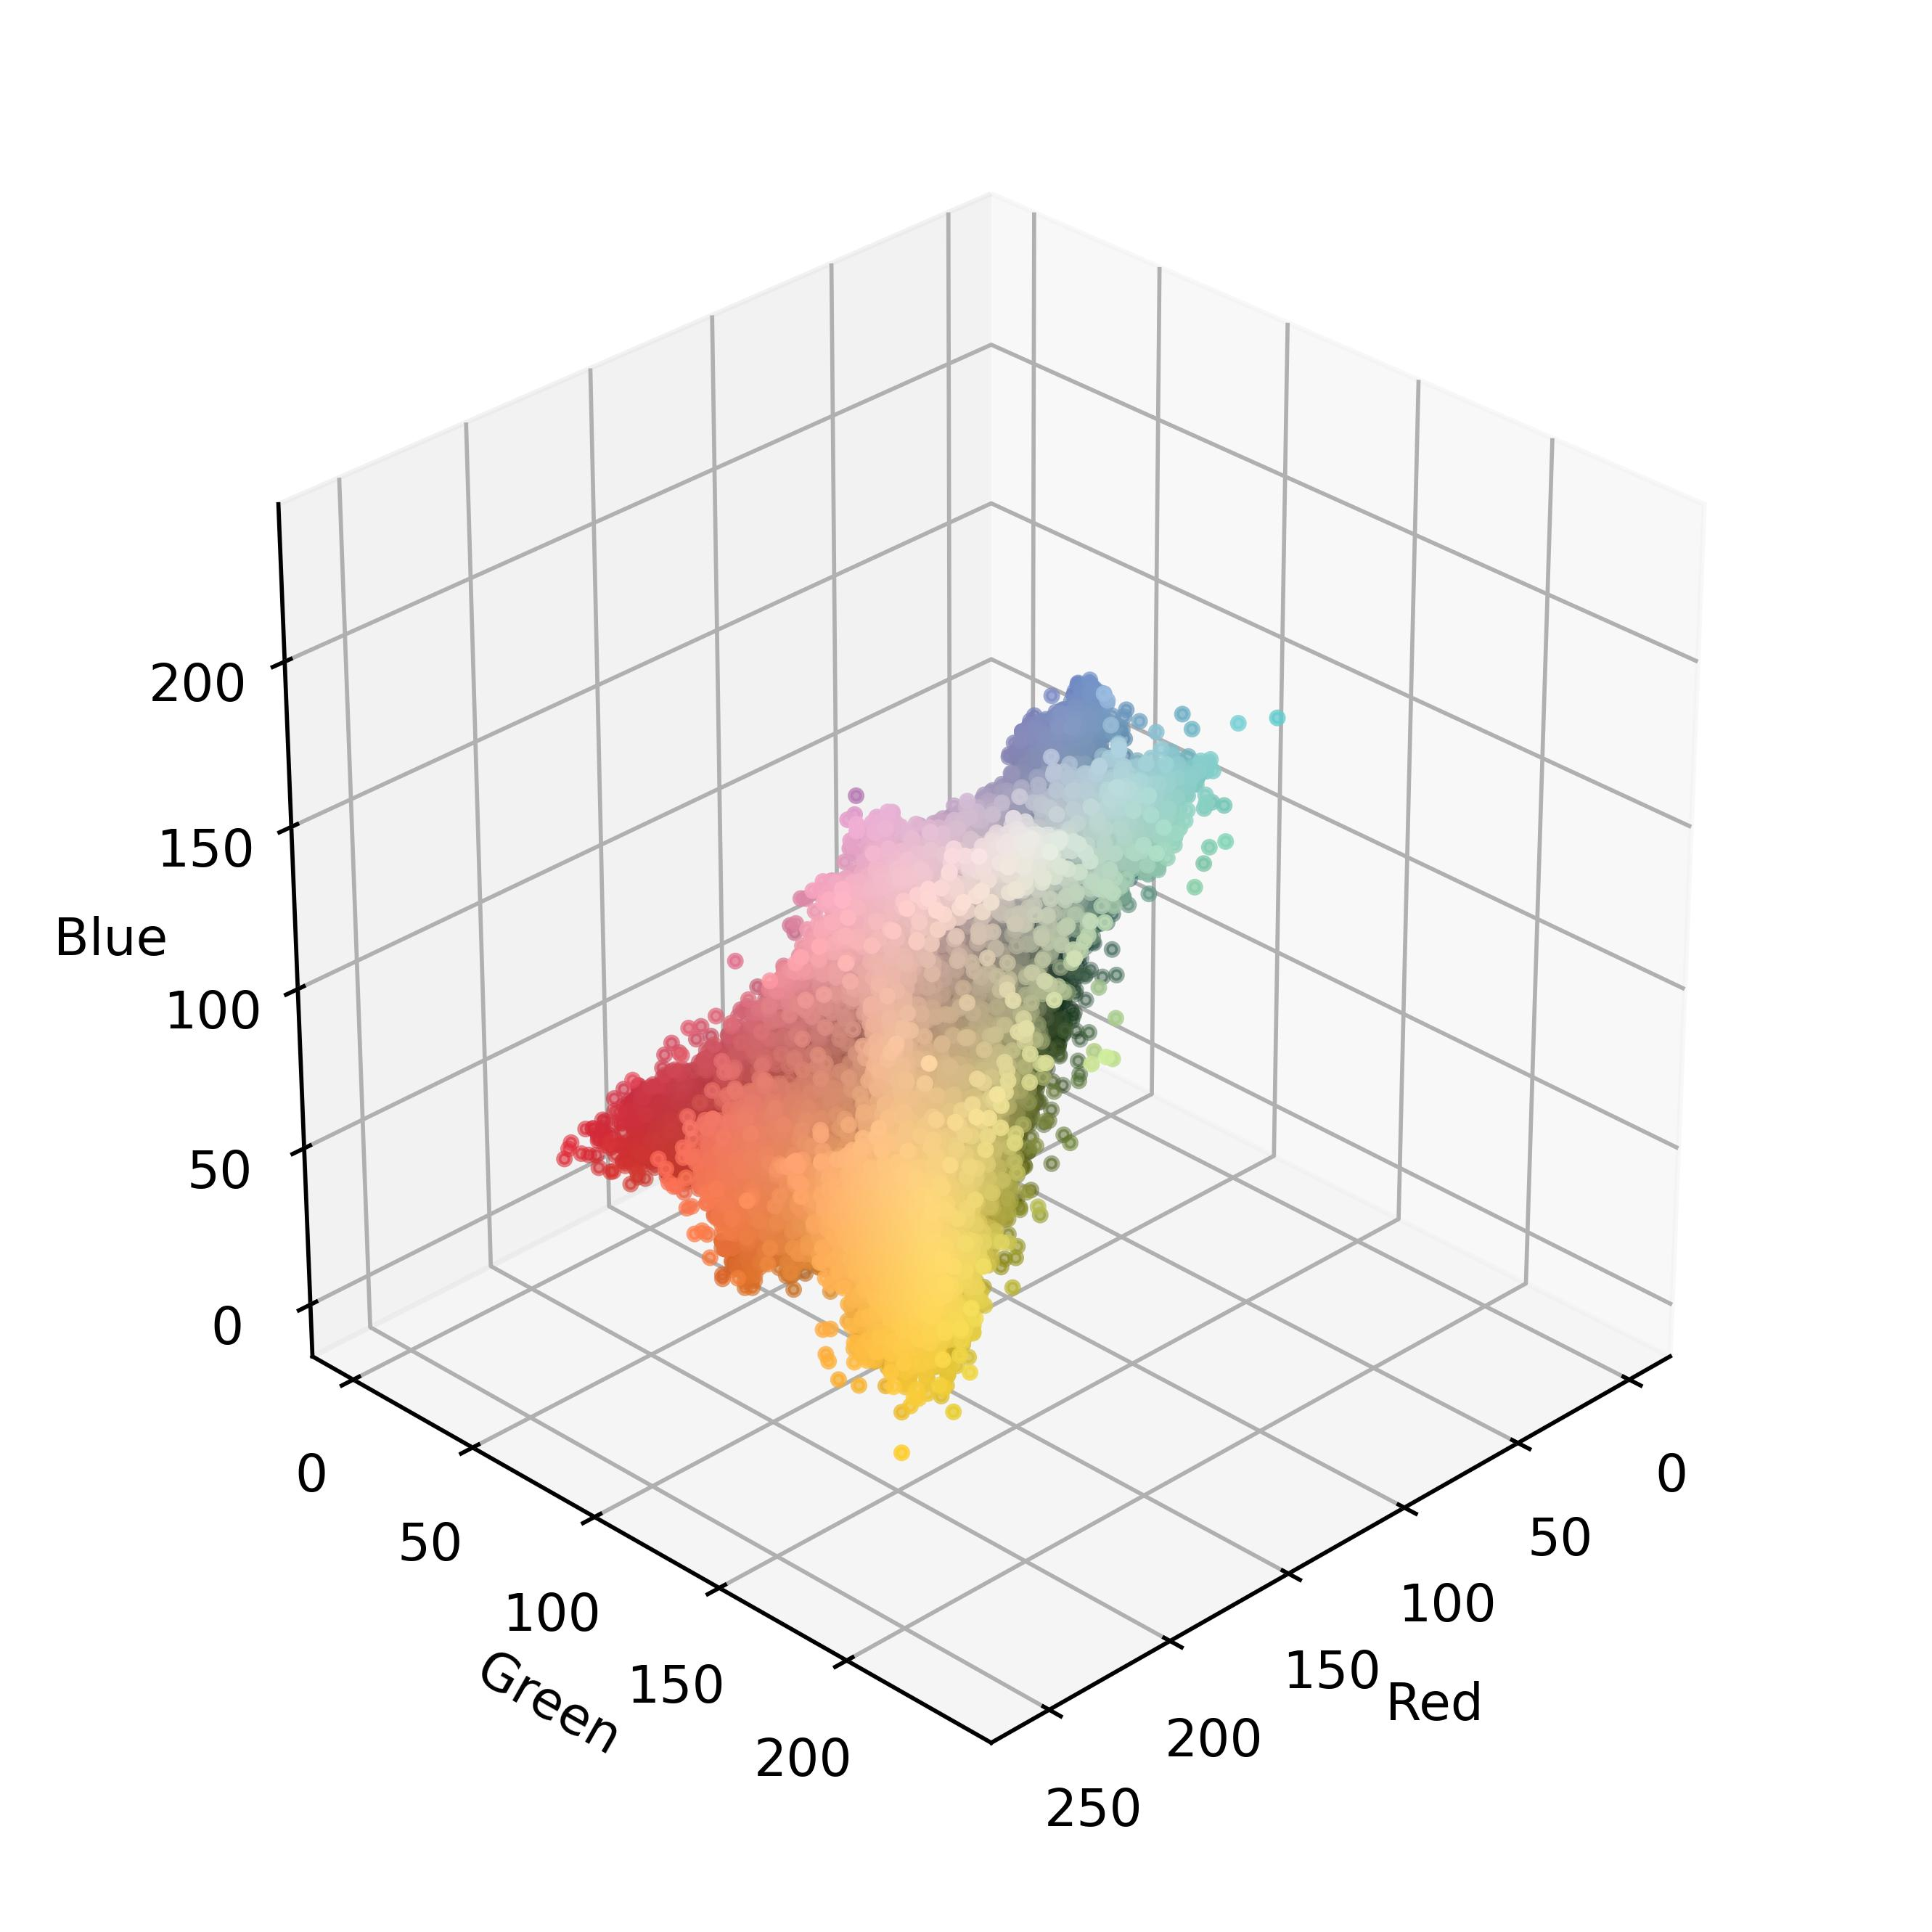
\includegraphics[width=\textwidth]{main_files/figure-latex/4_1_orange_marilyn_original_scatter.jpg}
    \caption{Figure 4.1: Orange Marilyn Angle 1}
    \label{fig:4_1_orange_marilyn_original_scatter}
  \end{subfigure}
  \hfill
  \begin{subfigure}{0.45\textwidth}
    \centering
    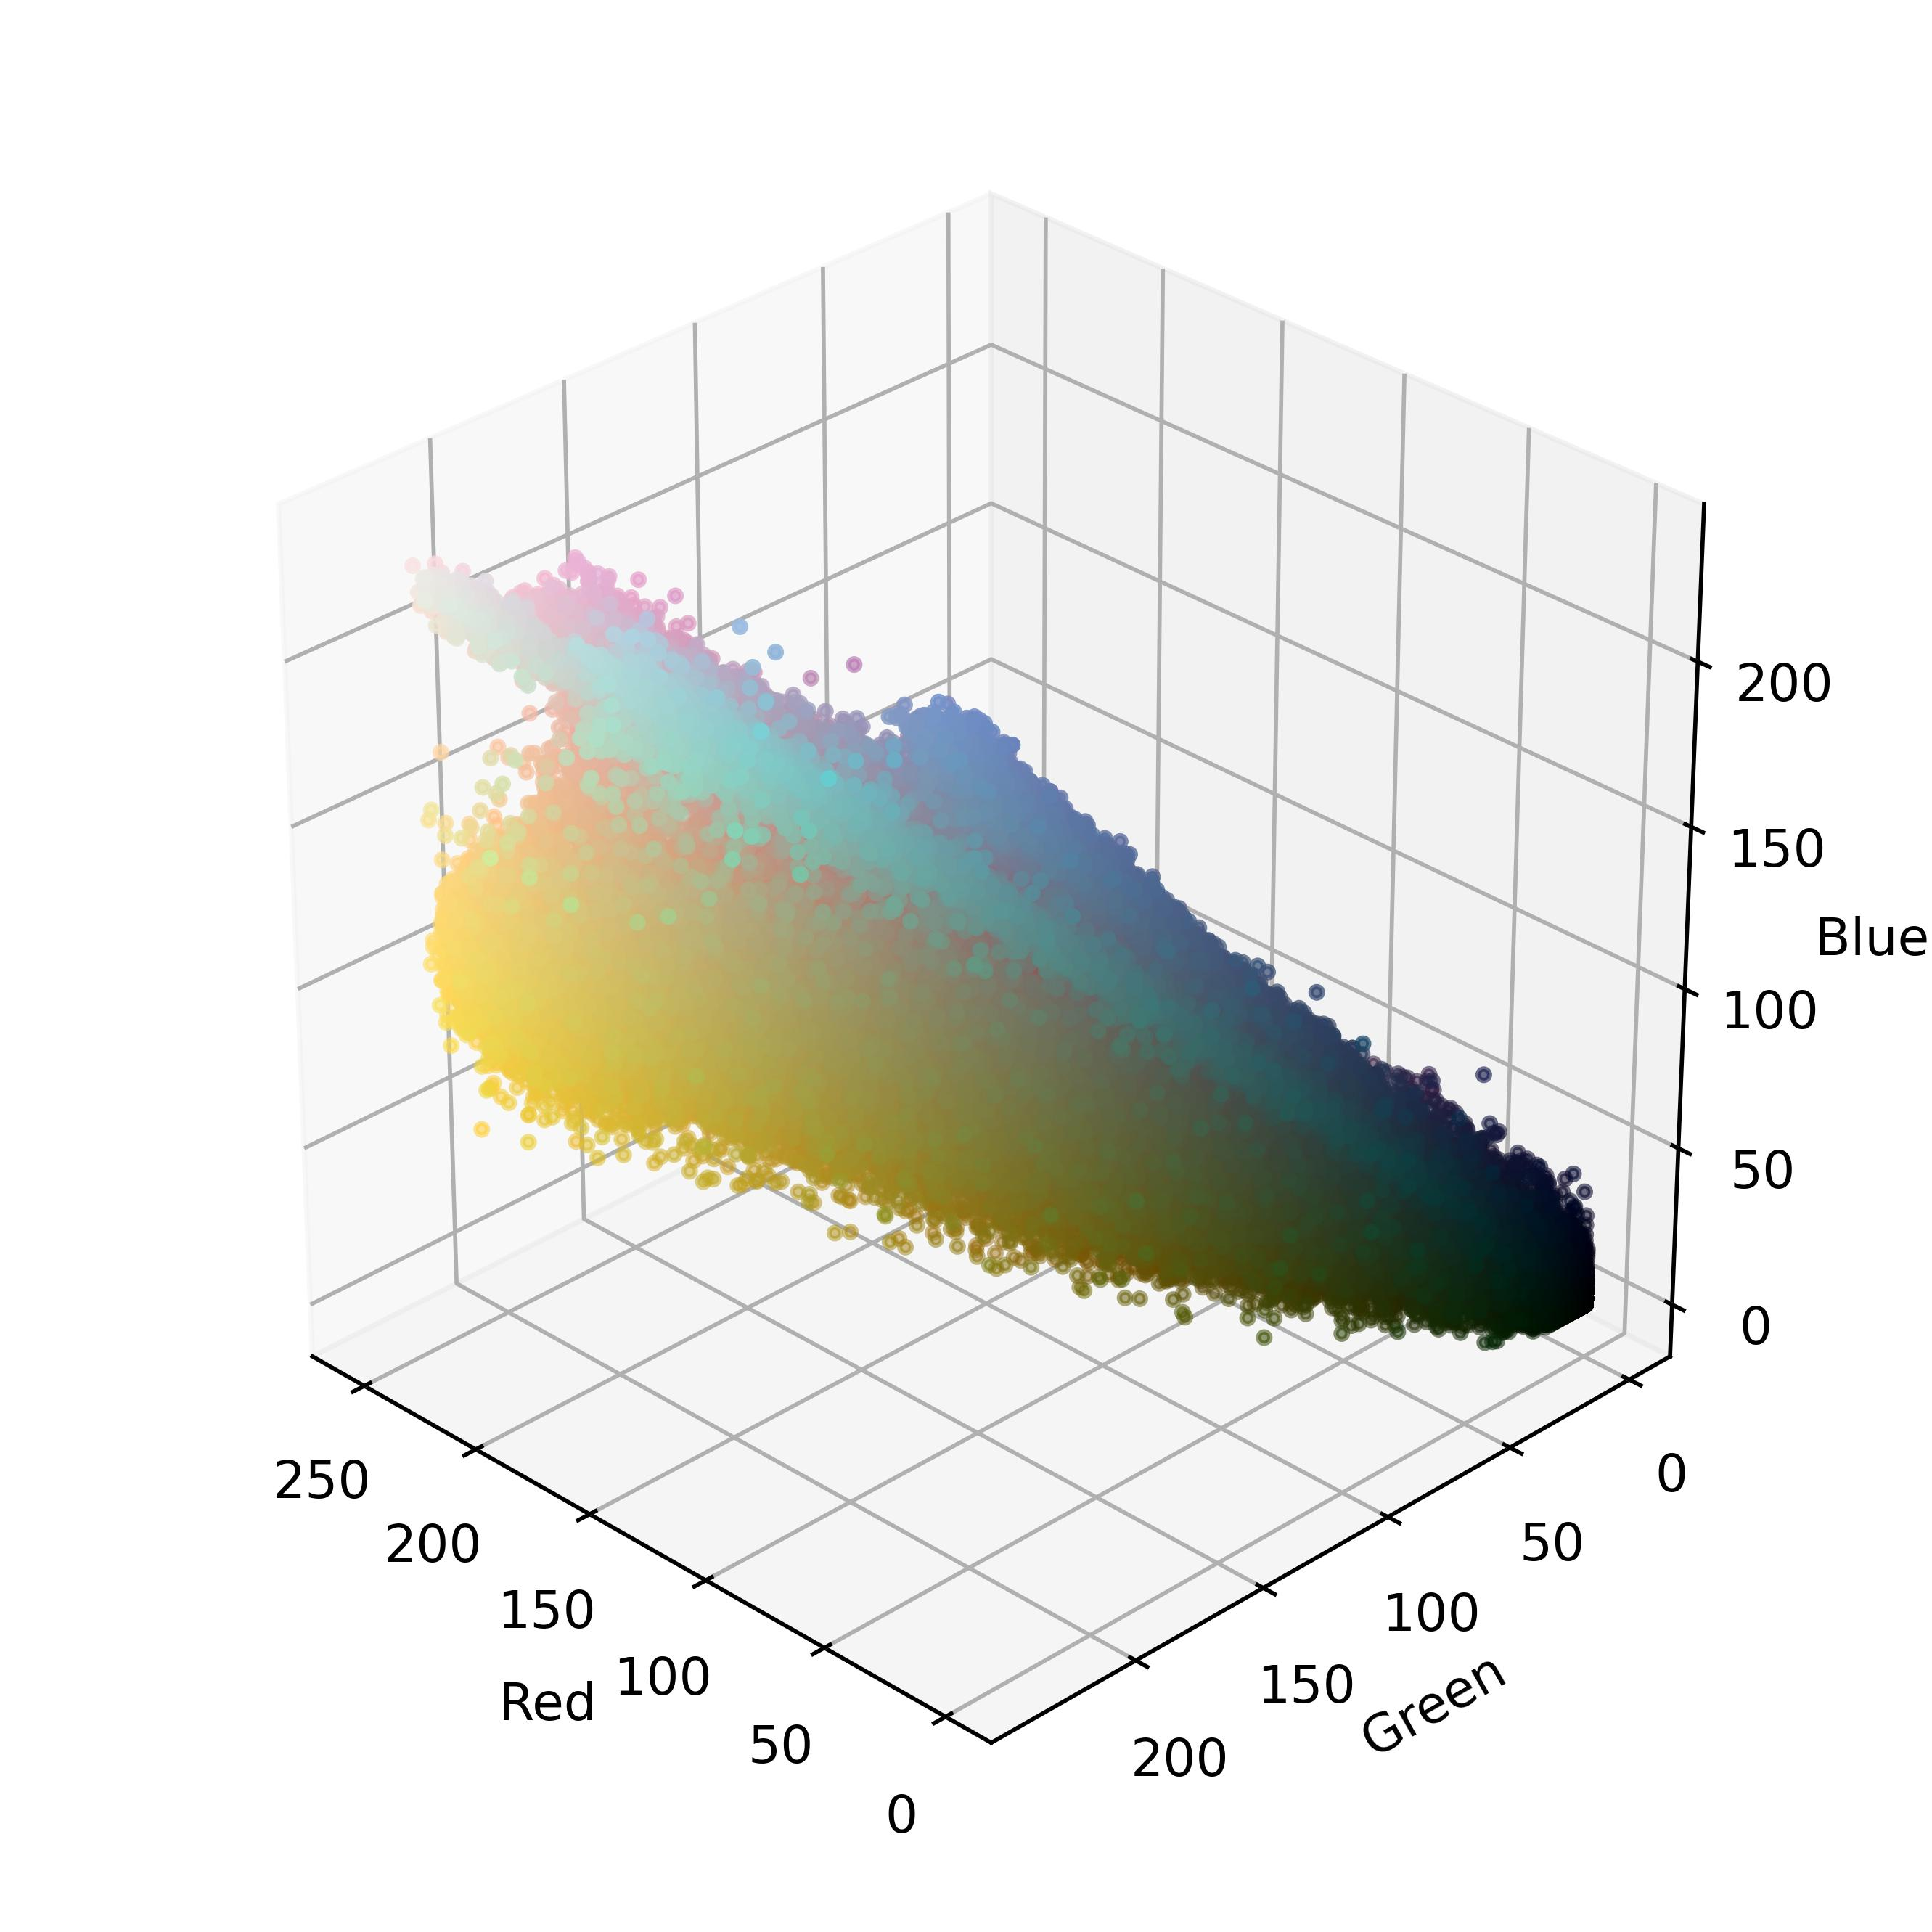
\includegraphics[width=\textwidth]{main_files/figure-latex/4_2_orange_marilyn_original_scatter.jpg}
    \caption{Figure 4.2: Orange Marilyn Angle 2}
    \label{fig:4_2_orange_marilyn_original_scatter}
  \end{subfigure}
  
  \vspace{1em}
  
  \begin{subfigure}{0.45\textwidth}
    \centering
    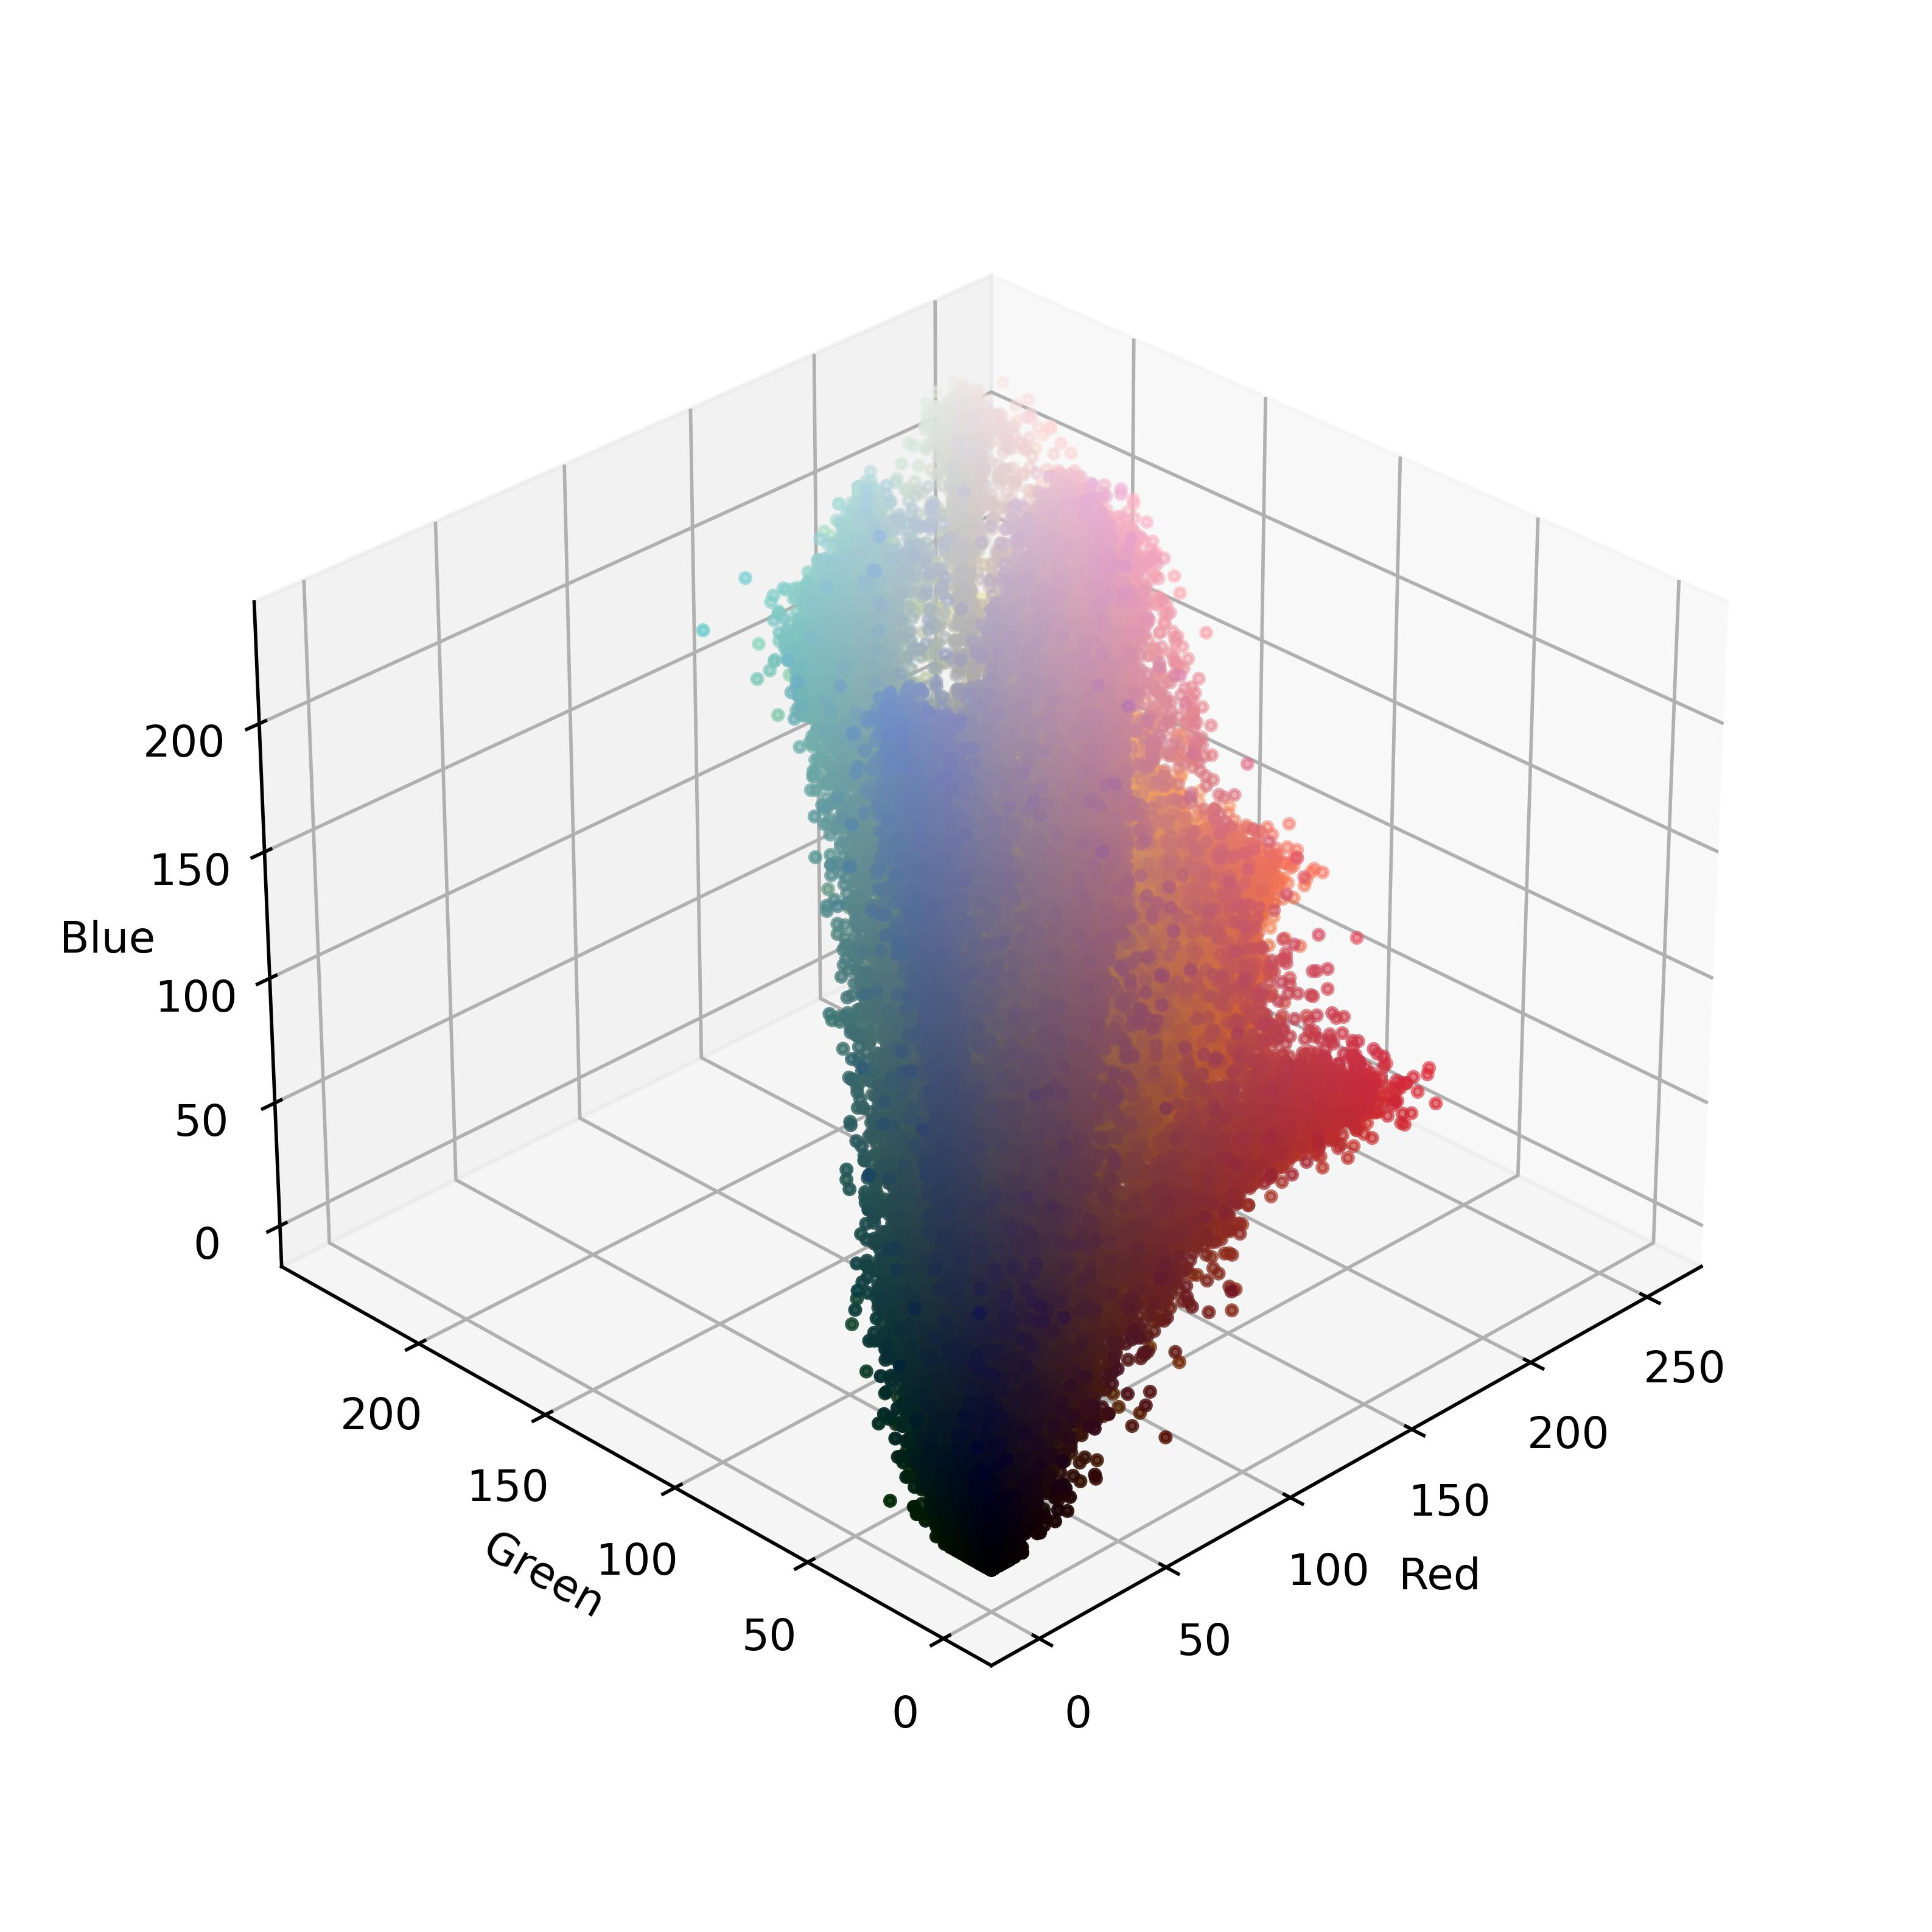
\includegraphics[width=\textwidth]{main_files/figure-latex/4_3_orange_marilyn_original_scatter.jpg}
    \caption{Figure 4.3: Orange Marilyn Angle 3}
    \label{fig:4_3_orange_marilyn_original_scatter}
  \end{subfigure}
  \hfill
  \begin{subfigure}{0.45\textwidth}
    \centering
    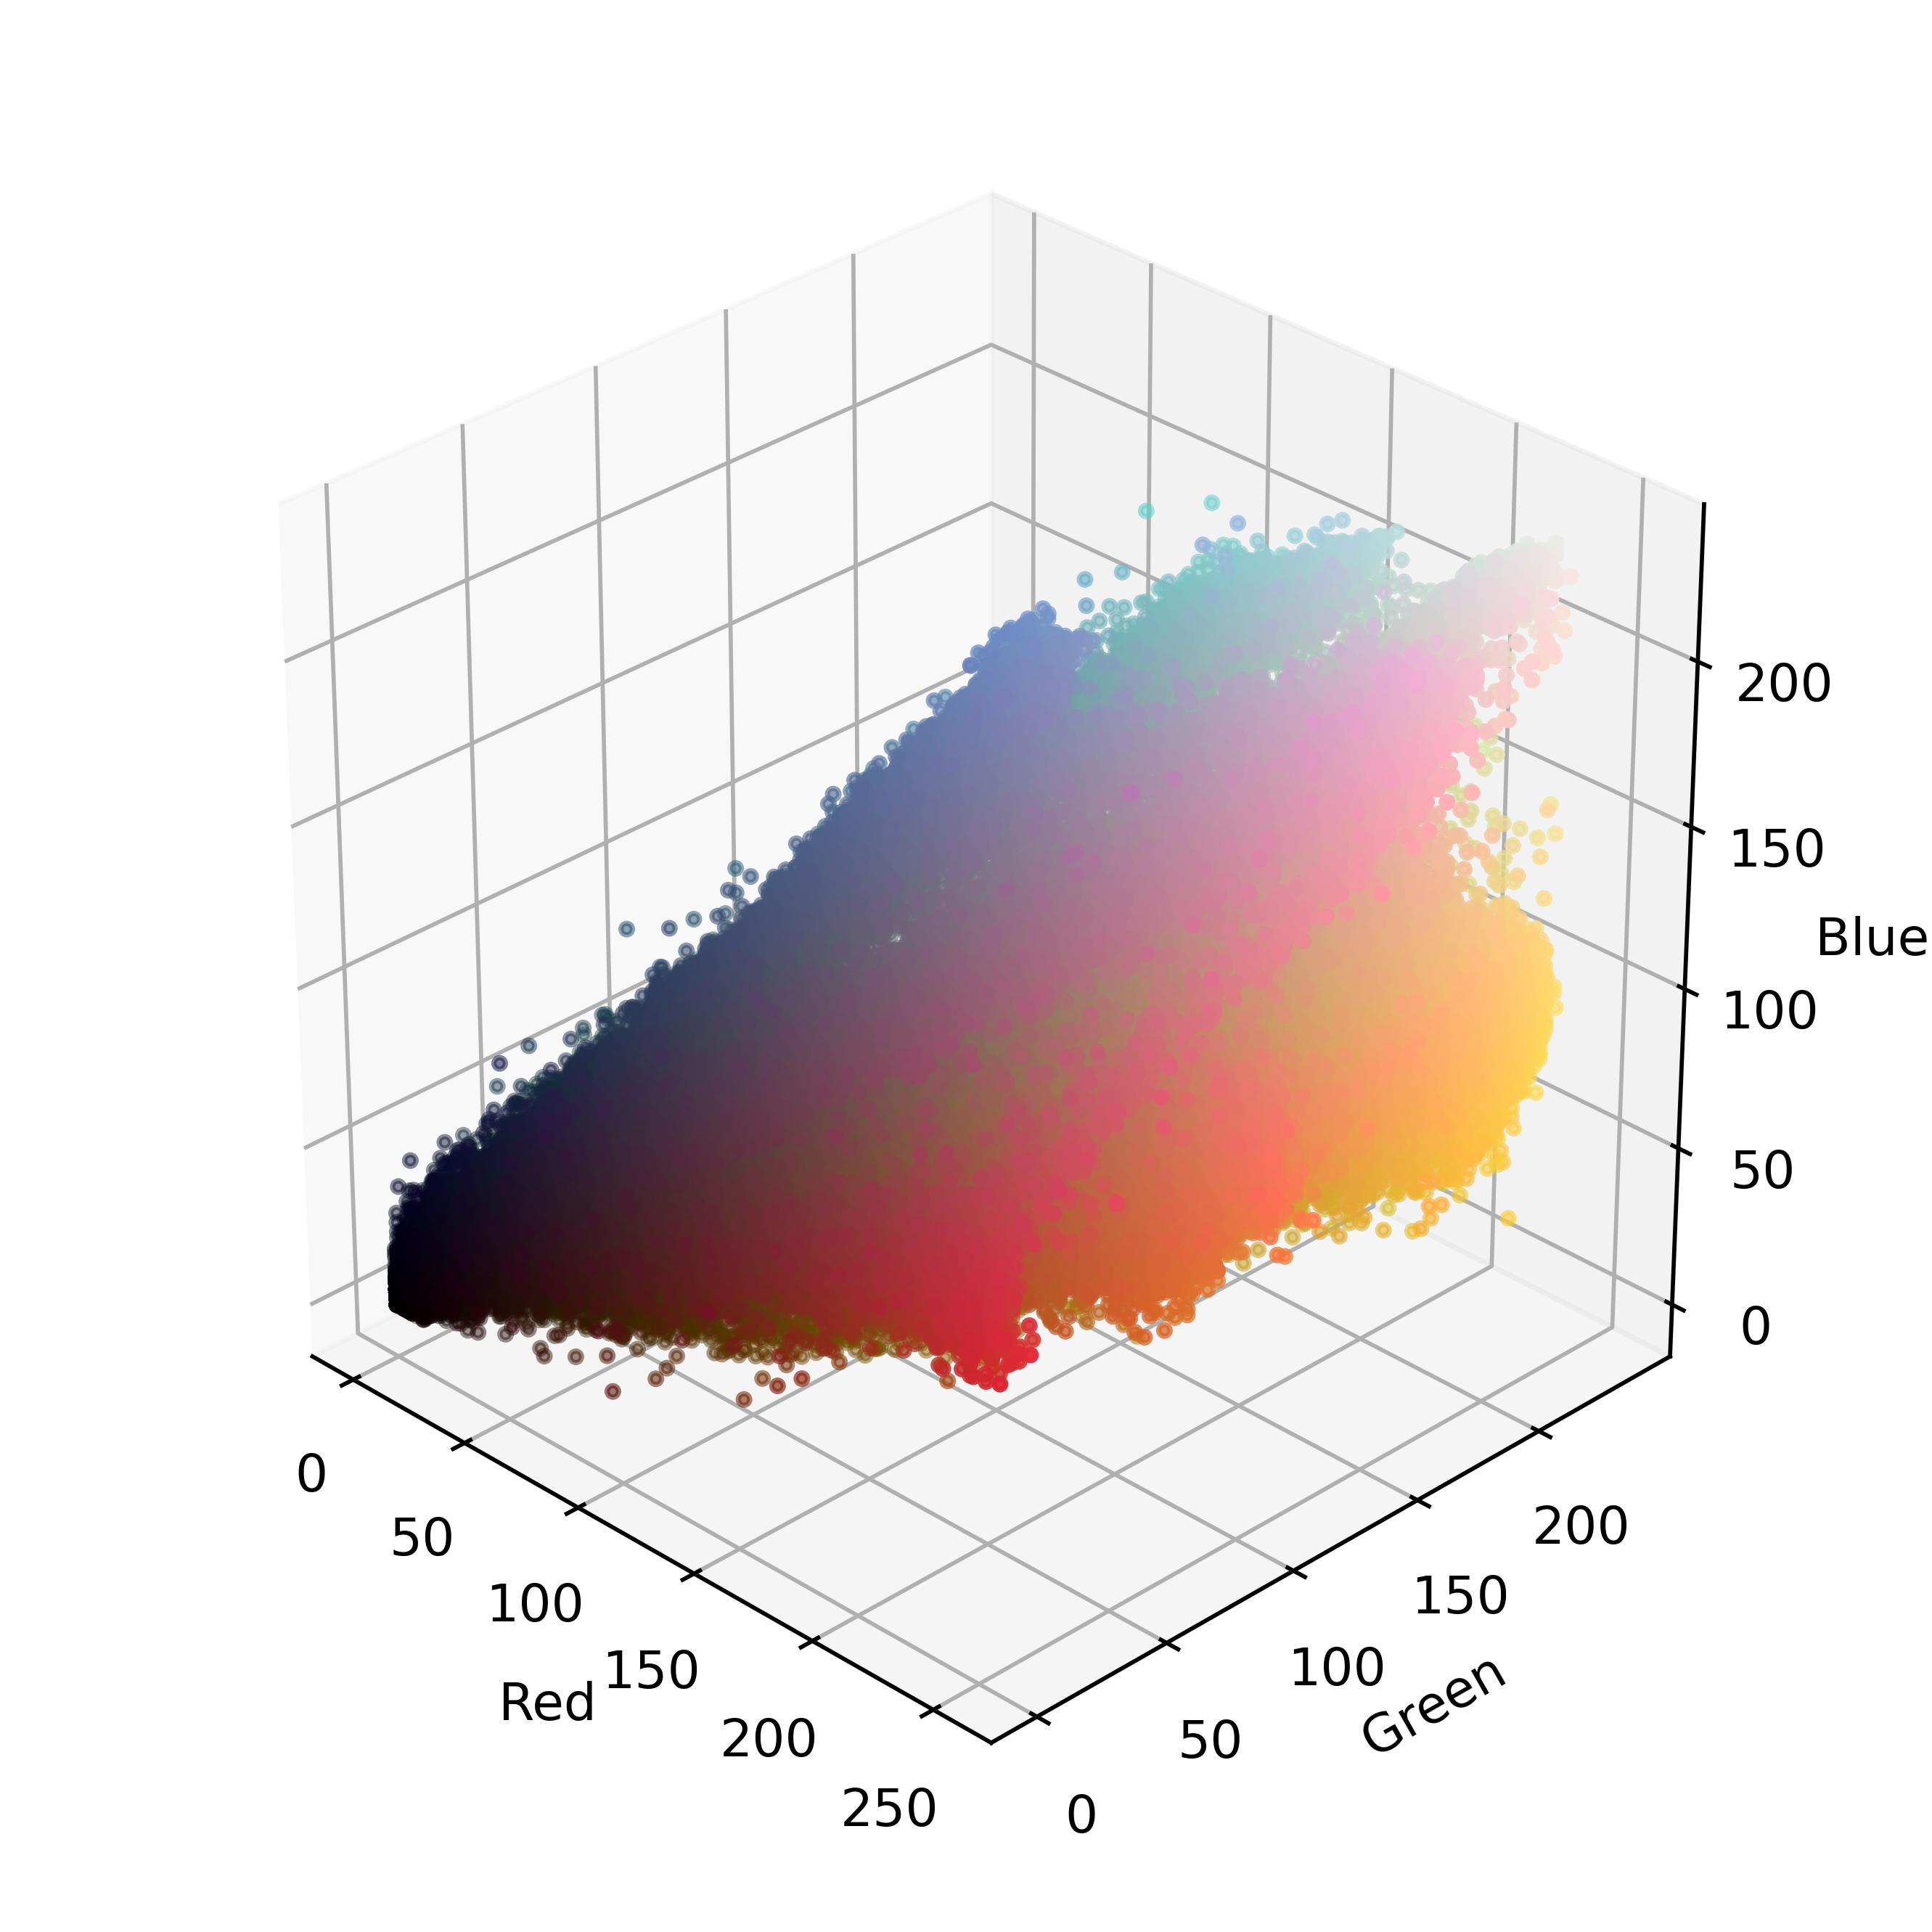
\includegraphics[width=\textwidth]{main_files/figure-latex/4_4_orange_marilyn_original_scatter.jpg}
    \caption{Figure 4.4: Orange Marilyn Angle 4}
    \label{fig:4_4_orange_marilyn_original_scatter}
  \end{subfigure}
  
  \caption{Scatter Plot of Orange Marilyn}
  \label{fig:orange_marilyn_scatter}
\end{figure}

In Figure 5, the four scatter plots depict the RGB color distribution
for the Orange painting of Marilyn Monroe. Top scatter plots s shows
Green vs.~Red, the middle plot displays Blue vs.~Red, and the right plot
presents Blue vs.~Green. Each point represents a pixel centroid in the
painting. We can observe that yellow and orange are prominent across all
scatter plots. The bottom three graphs replicate the top three scatter
plots but use grayscale to represent the intensity of the absent color.
In the left plot, darker points indicate a higher presence of blue; in
the middle plot, darker points signify a greater prominence of green;
and in the right plot, darker points represent the prominence of red.

In the left and middle scatter plots, the most significant presence of
blue and green is concentrated near the right corner of the graph but is
not very prominent overall. In contrast, the right scatter plot shows
darker points throughout, indicating a substantial presence of red. This
observation aligns with the painting's color scheme, featuring an orange
background and yellow hair, both of which require a high content of red.

Rewrite:``Figure 4 illustrates the RGB color distribution for Andy
Warhol's Orange Marilyn painting through four scatter plots from
different angles. Each plot represents the intensity distribution of the
red, green, and blue channels, with each point in the painting. The
scatter plots reveal a predominant presence of yellow and orange hues,
reflecting the painting's color scheme of an orange background and
yellow hair, which requires a high red content. Notably, Figure 4.1 and
Figure 4.2 emphasize the horizontal and diagonal spread of colors, while
Figure 4.3 and Figure 4.4 highlight the vertical distribution, showing
significant concentrations of red and blue. These visualizations
collectively demonstrate the intricate balance of colors in Warhol's
work, showcasing the dynamic interplay and prominence of specific hues
that contribute to the painting's iconic visual impact.''

\begin{figure}[ht]
  \centering
  \begin{subfigure}{0.45\textwidth}
    \centering
    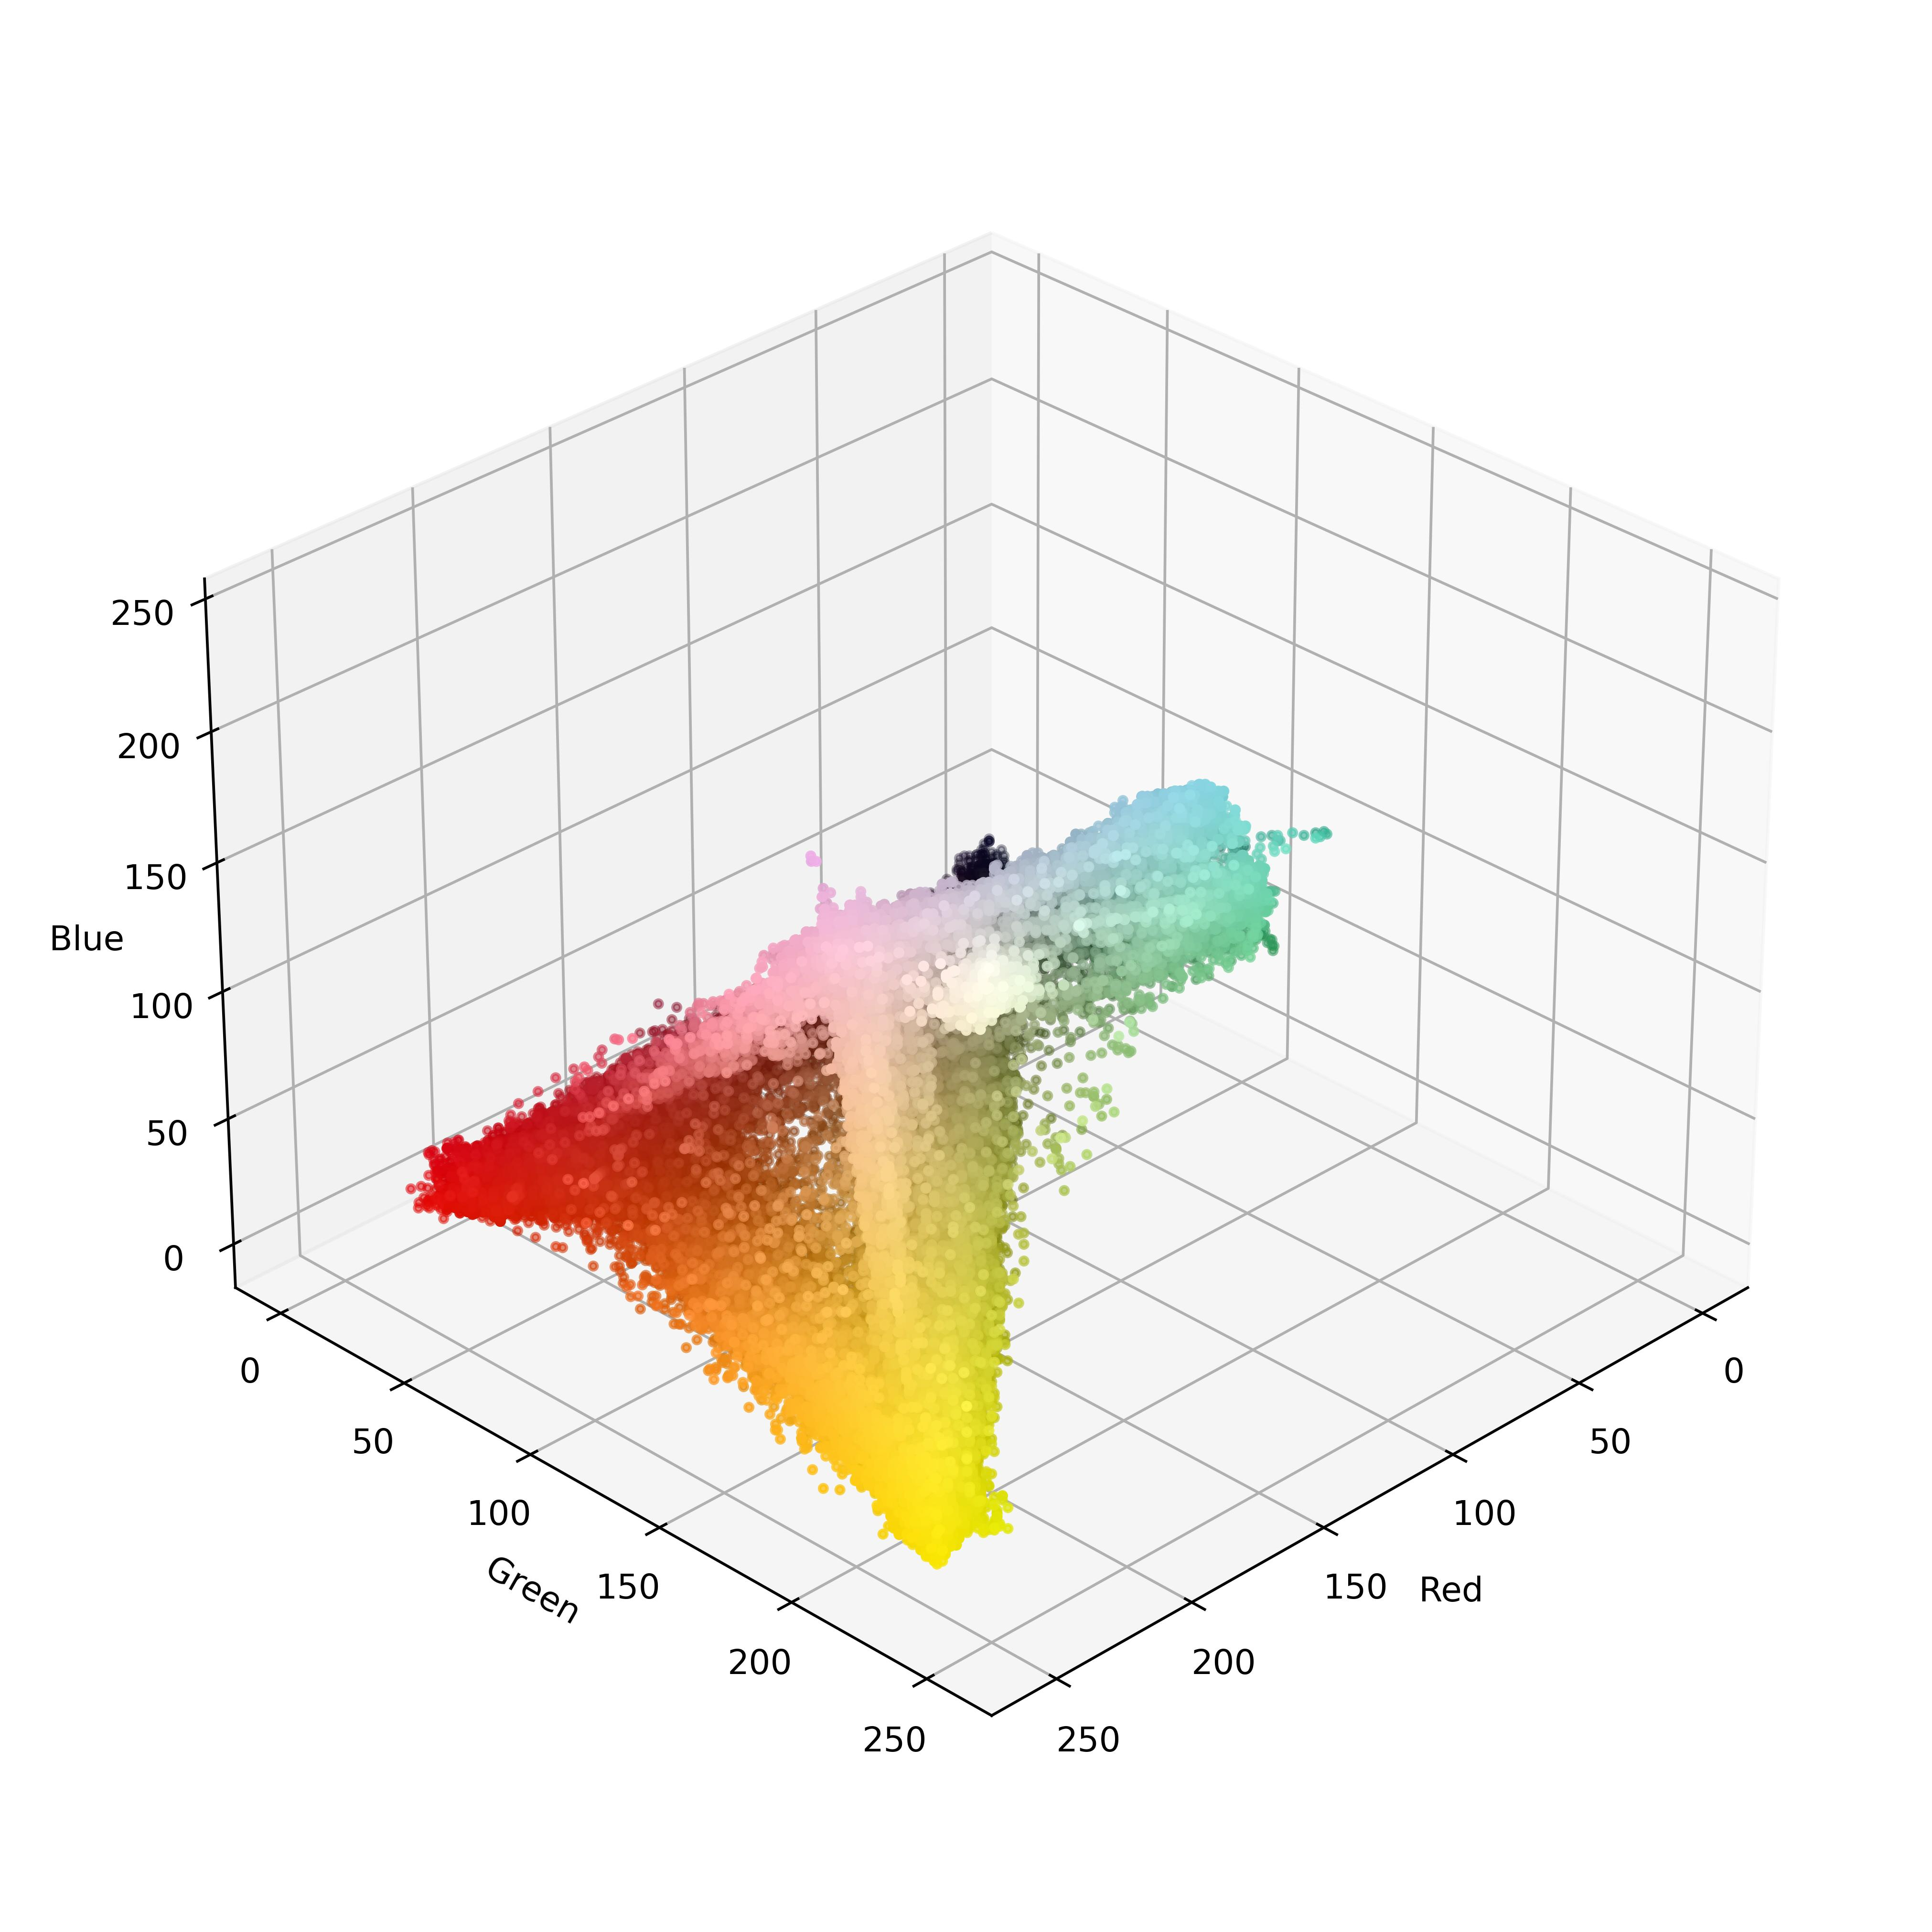
\includegraphics[width=\textwidth]{main_files/figure-latex/4_5_red_marilyn_original_scatter.jpg}
    \caption{Figure 4.6: Red Marilyn Angle 1}
    \label{fig:4_6_red_marilyn_original_scatter}
  \end{subfigure}
  \hfill
  \begin{subfigure}{0.45\textwidth}
    \centering
    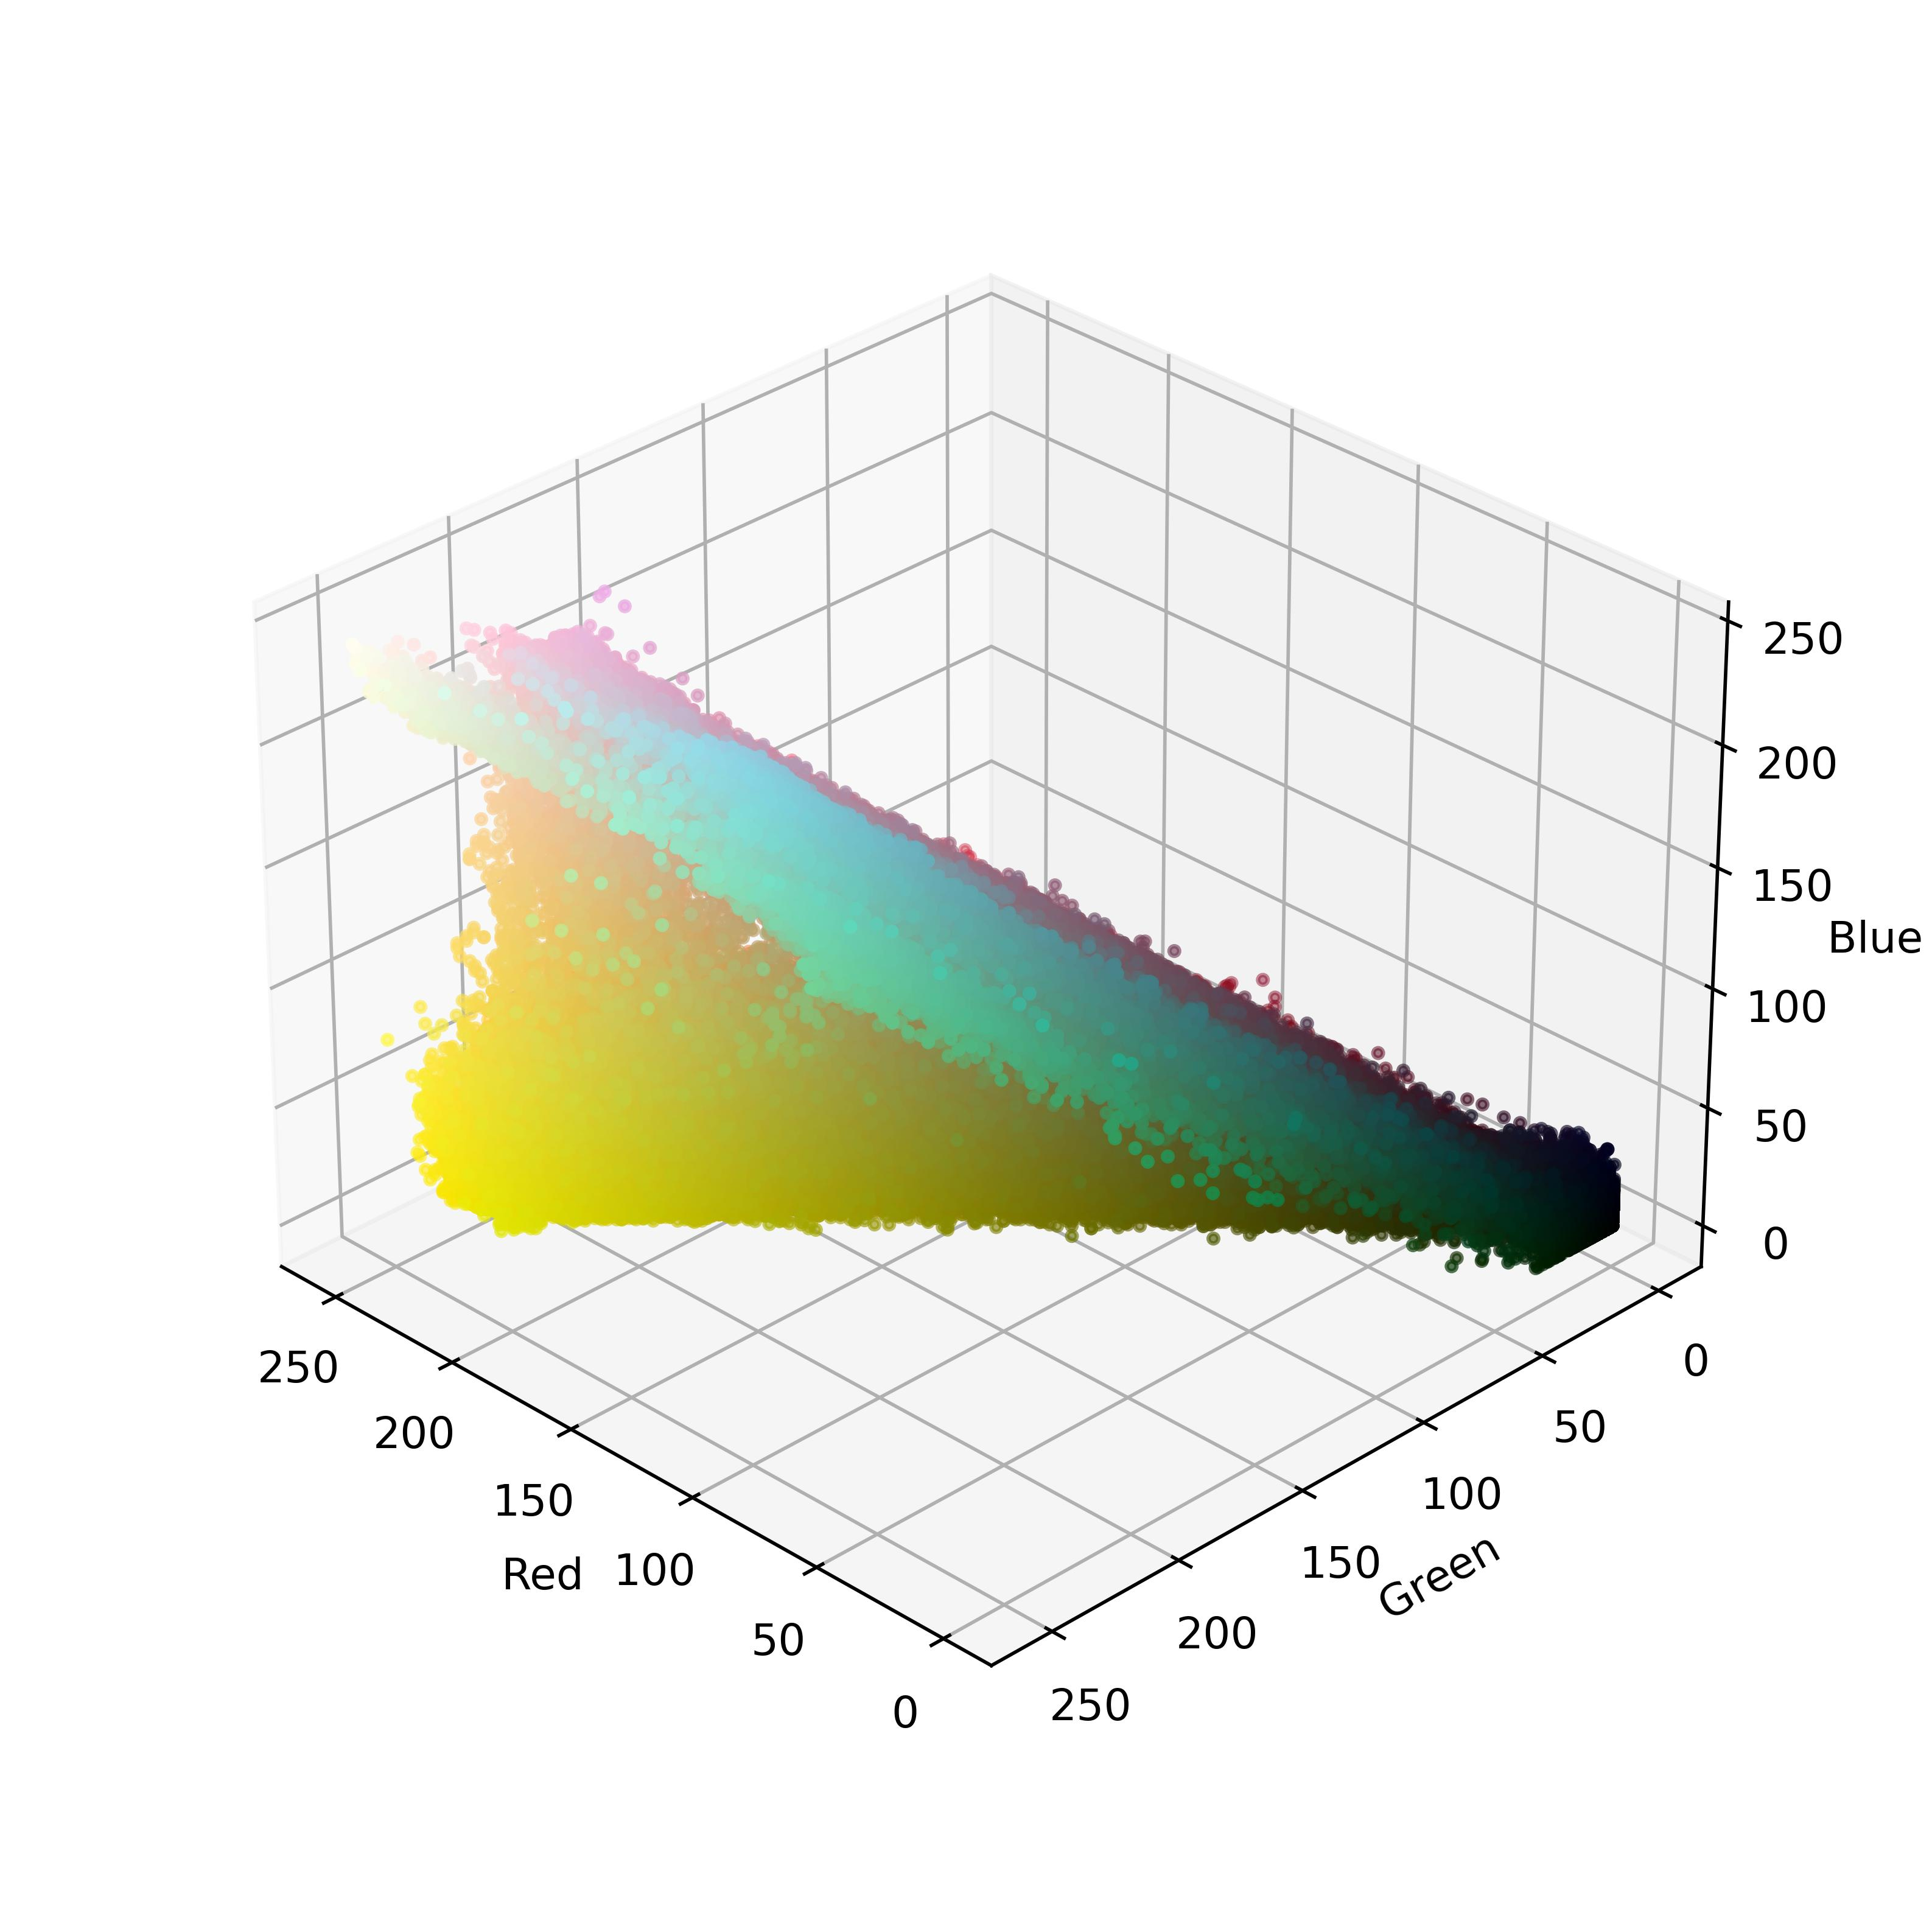
\includegraphics[width=\textwidth]{main_files/figure-latex/4_6_red_marilyn_original_scatter.jpg}
    \caption{Figure 4.7: Red Marilyn Angle 2}
    \label{fig:4_7_red_marilyn_original_scatter}
  \end{subfigure}
  
  \vspace{1em}
  
  \begin{subfigure}{0.45\textwidth}
    \centering
    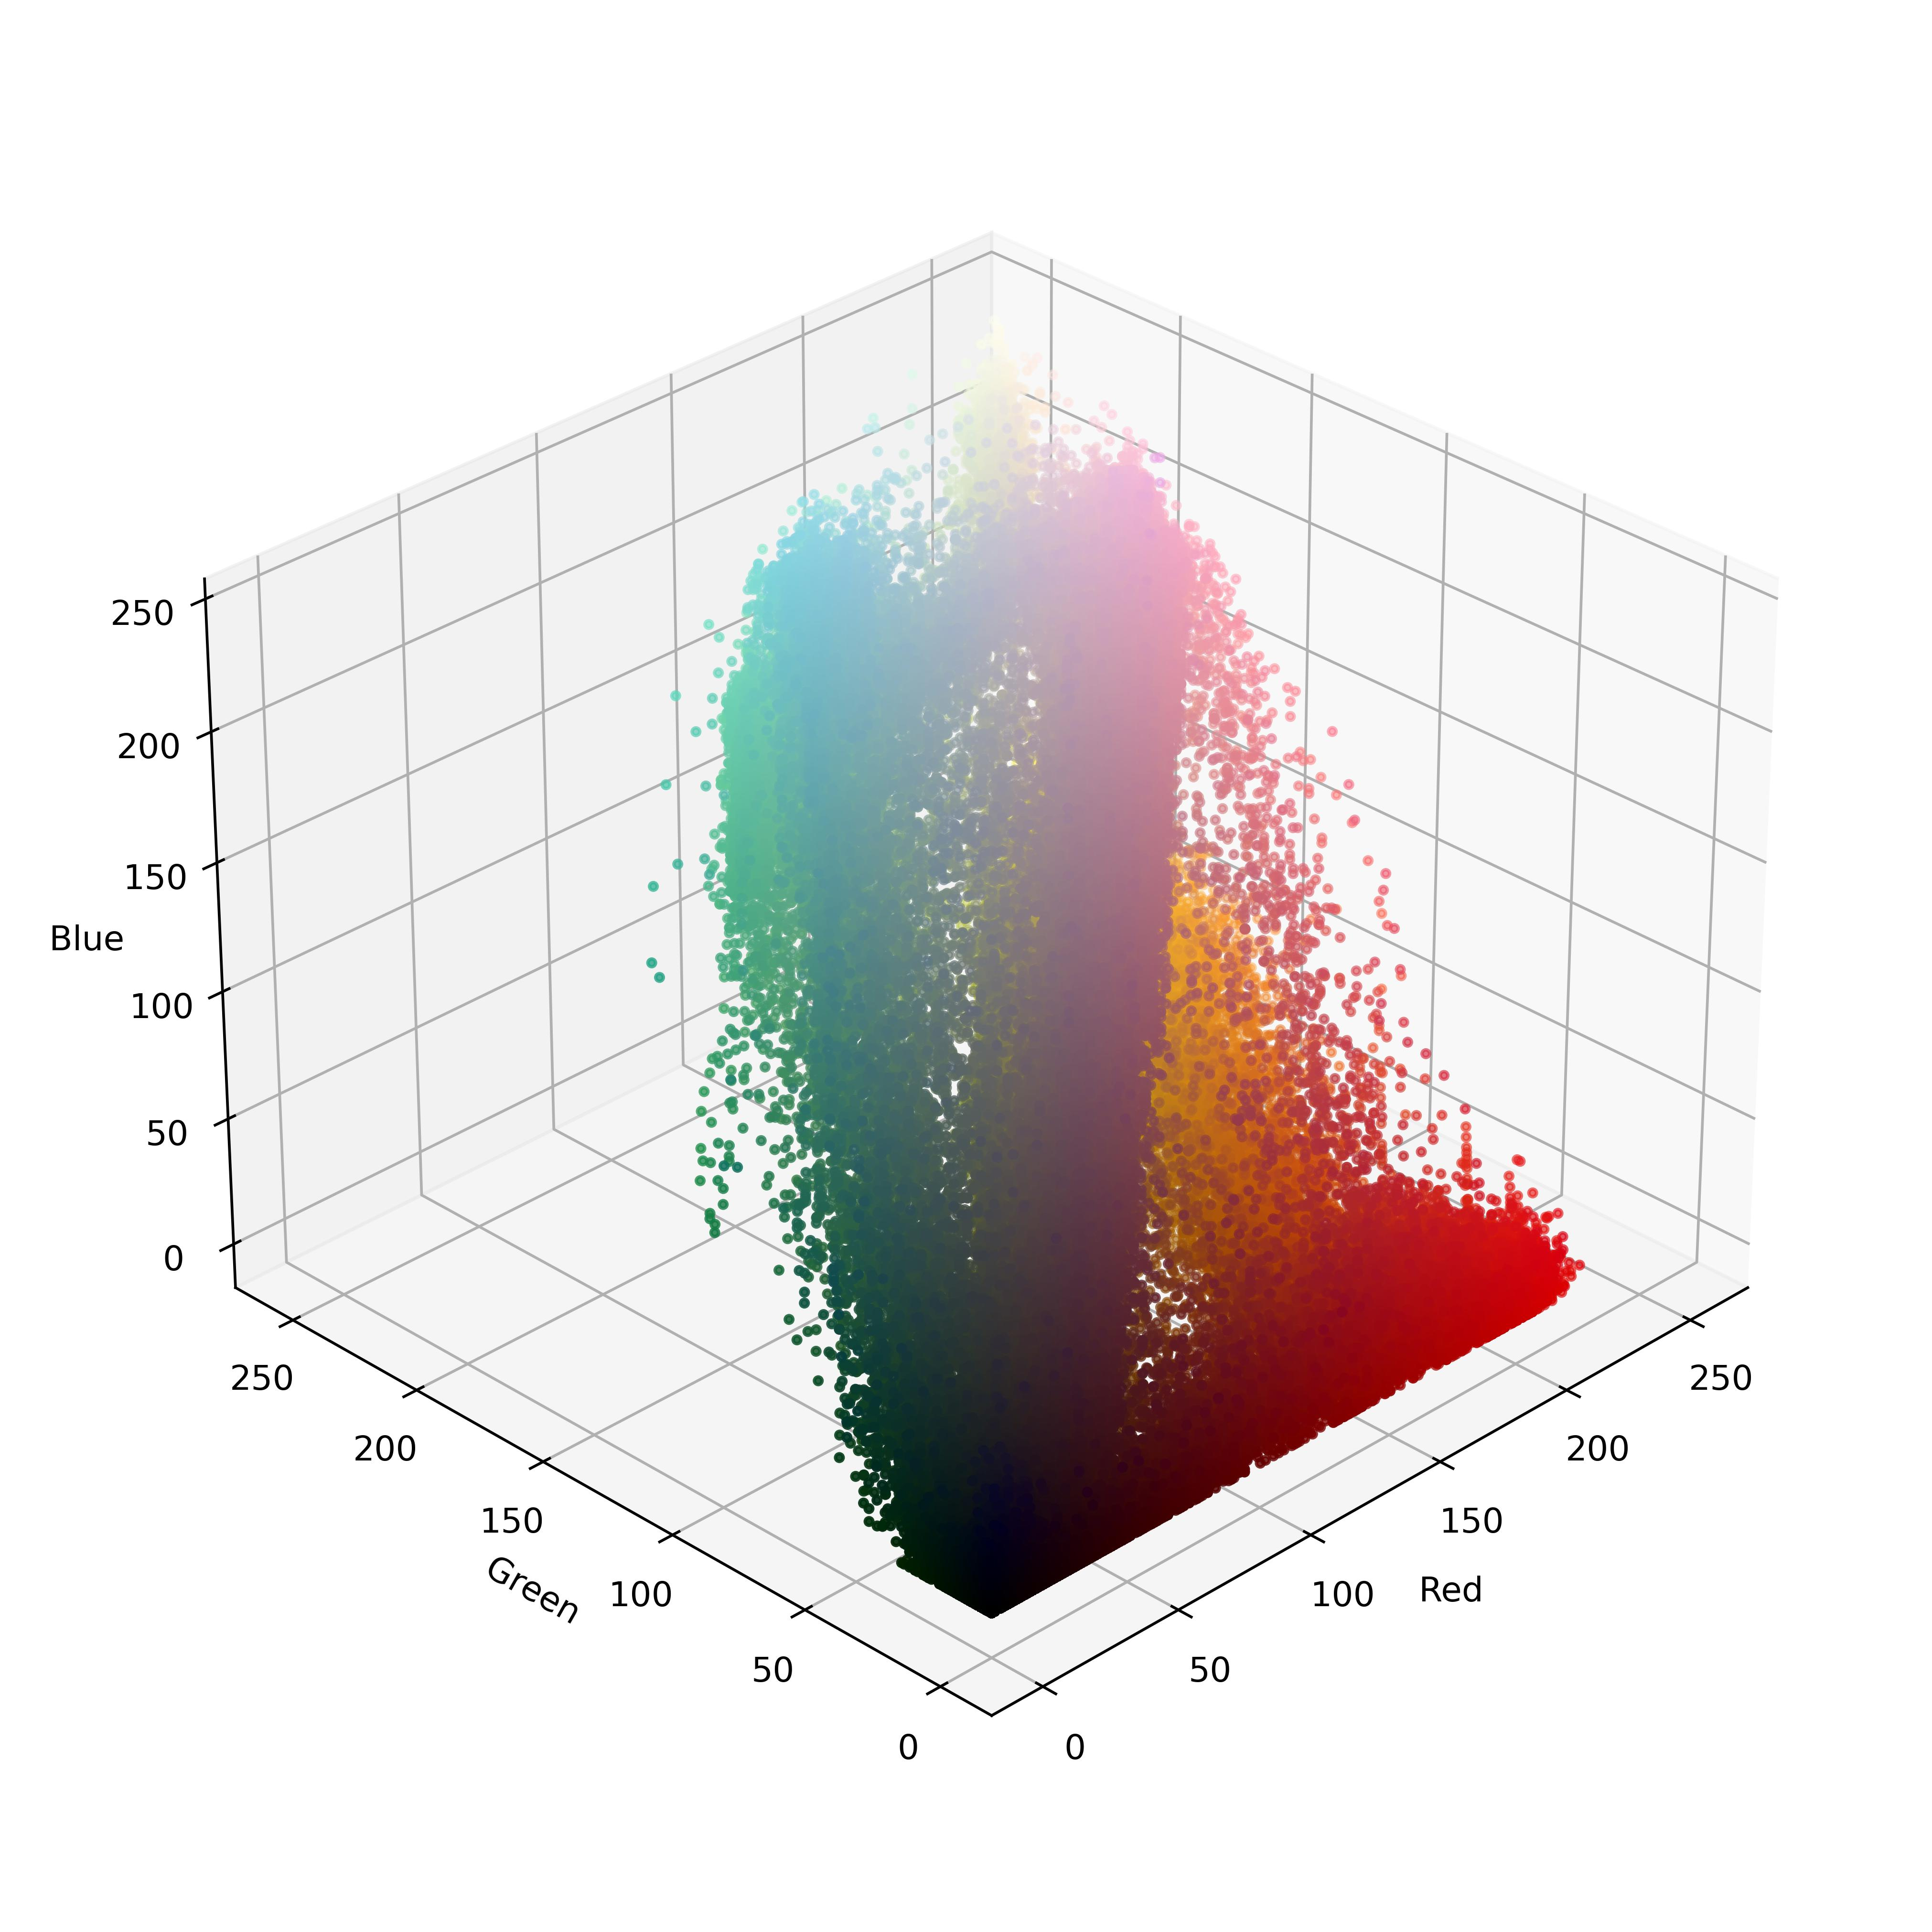
\includegraphics[width=\textwidth]{main_files/figure-latex/4_7_red_marilyn_original_scatter.jpg}
    \caption{Figure 4.8: Red Marilyn Angle 3}
    \label{fig:4_8_red_marilyn_original_scatter}
  \end{subfigure}
  \hfill
  \begin{subfigure}{0.45\textwidth}
    \centering
    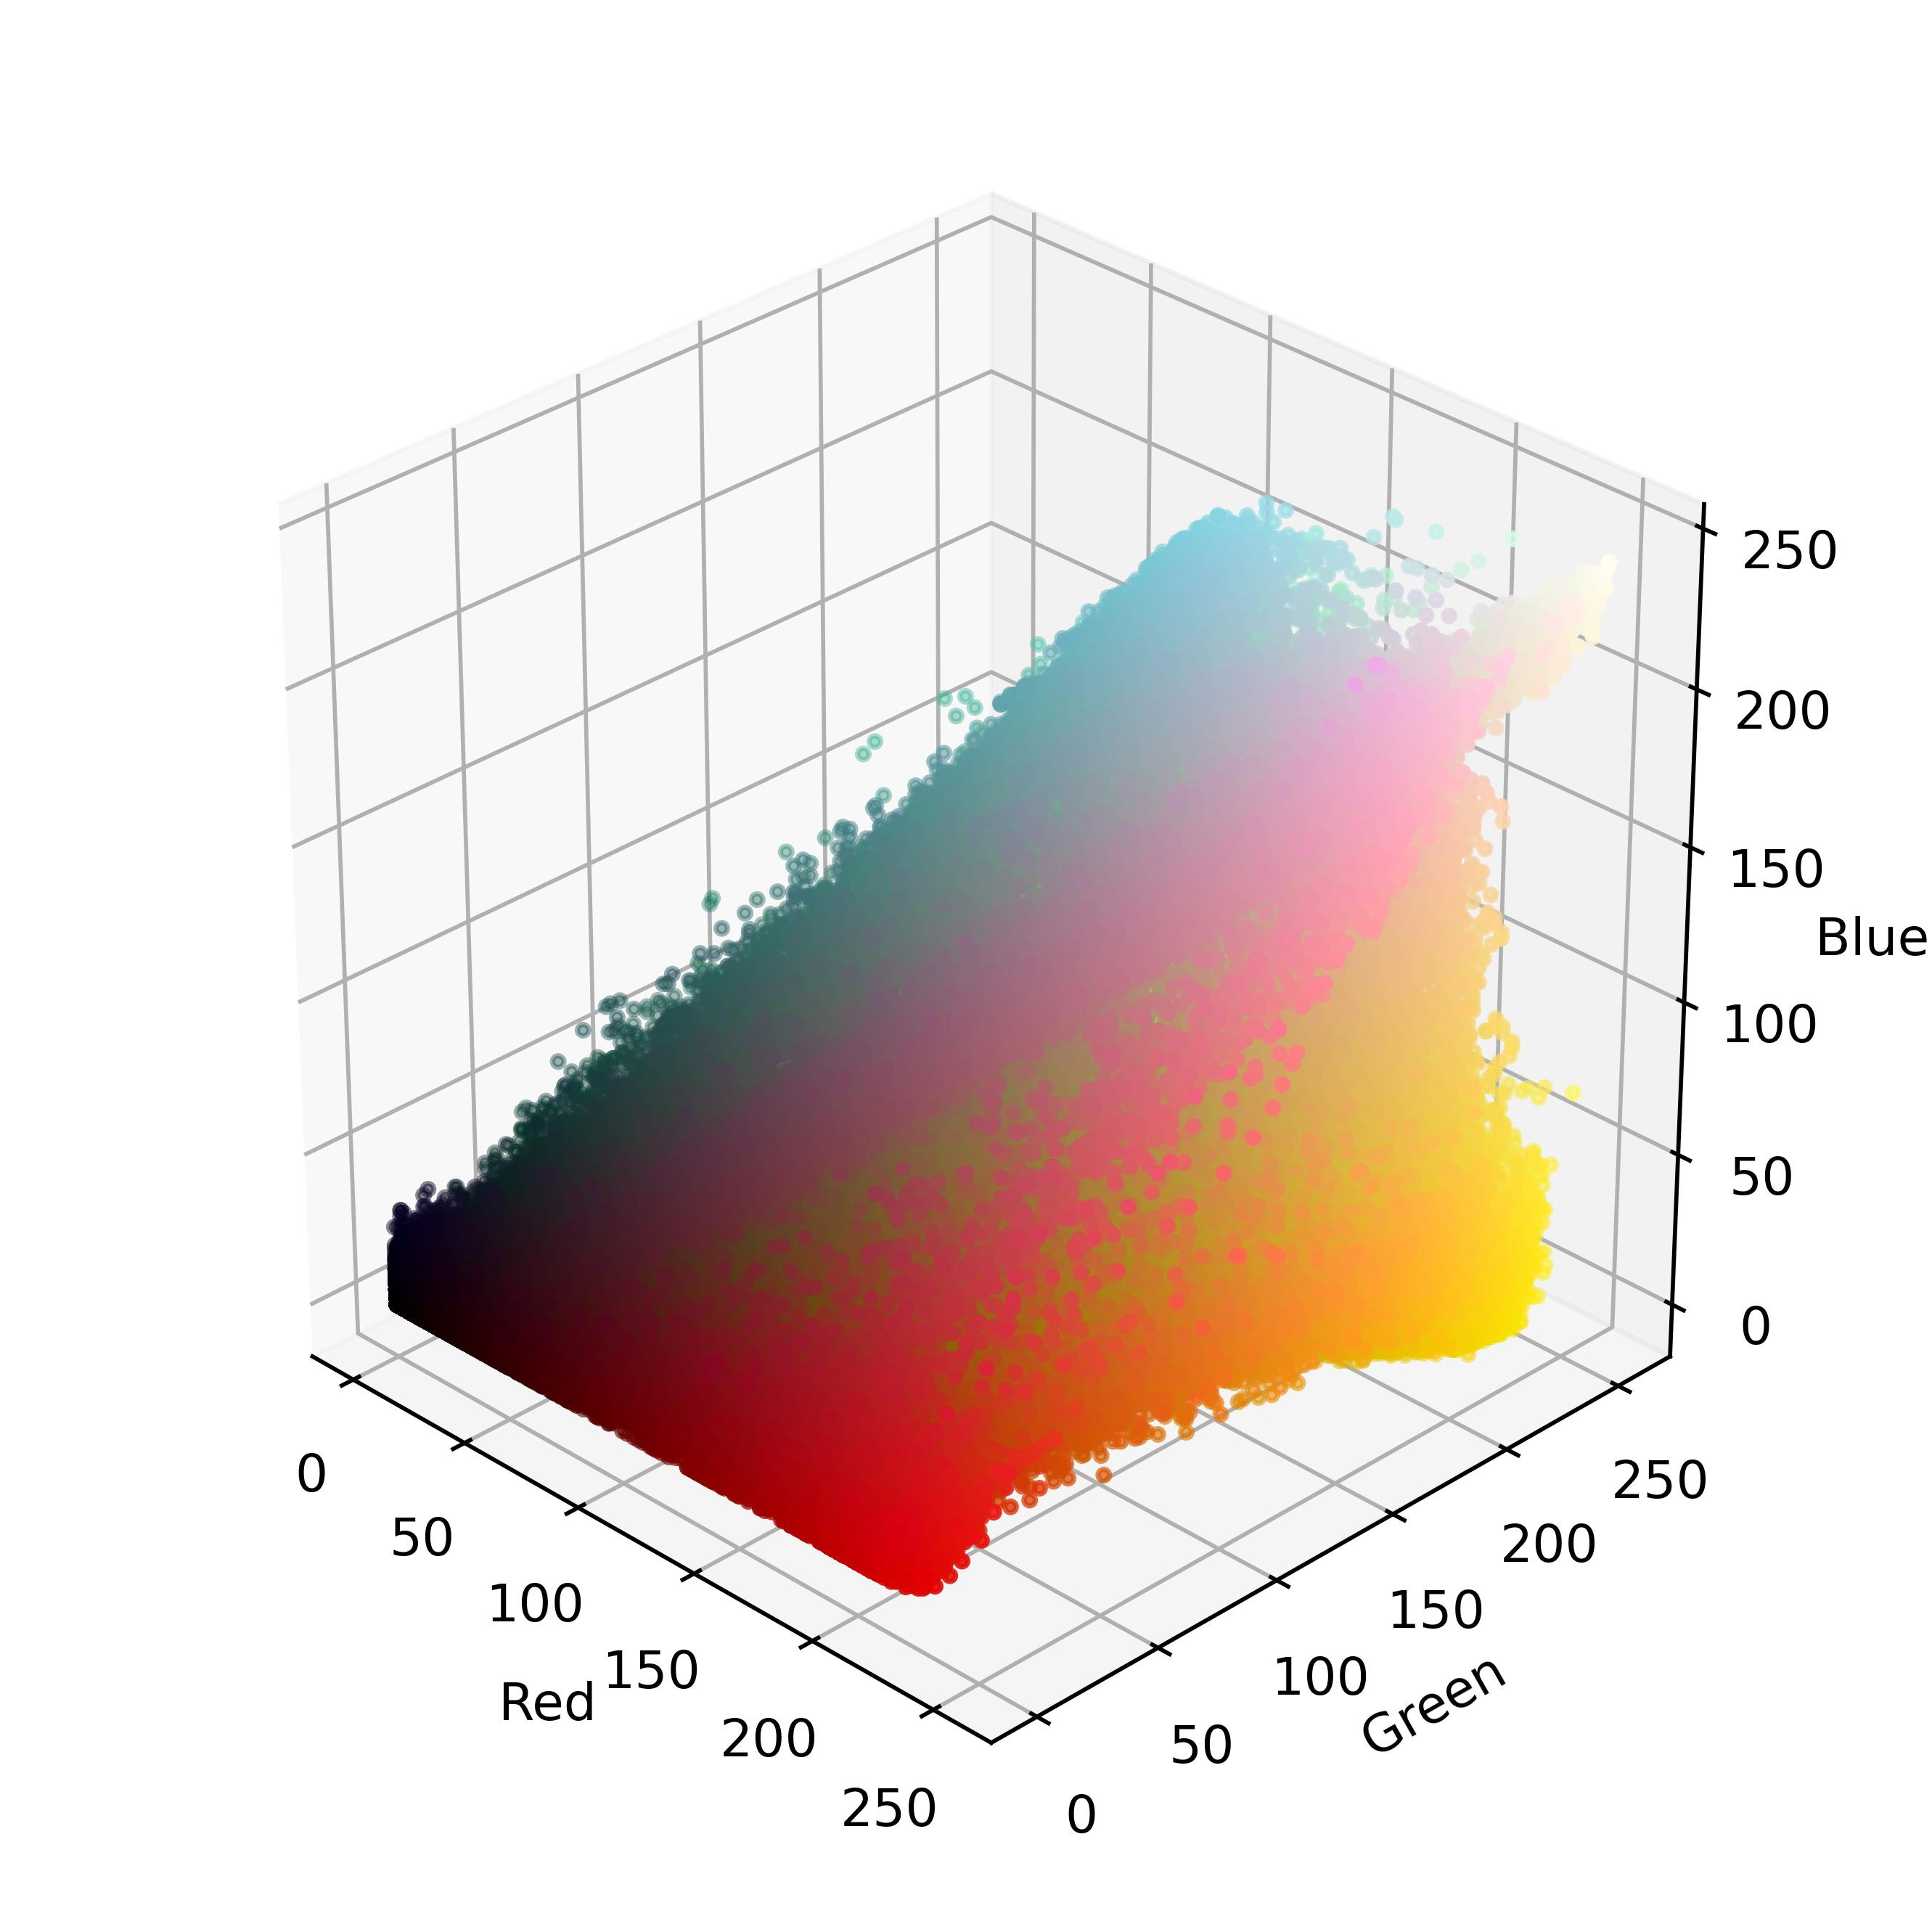
\includegraphics[width=\textwidth]{main_files/figure-latex/4_8_red_marilyn_original_scatter.jpg}
    \caption{Figure 4.9: Red Marilyn Angle 4}
    \label{fig:4_9_red_marilyn_original_scatter}
  \end{subfigure}
  
  \caption{Scatter Plot of Red Marilyn}
  \label{fig:orange_marilyn_scatter}
\end{figure}

In Figure 6, the top three scatter plots show the color distribution for
the Red shot of Marilyn Monroe. The left plot represents Green vs.~Red,
the center plot shows Blue vs.~Red, and the right plot displays Blue
vs.~Green. Although the presence of all colors makes it challenging to
interpret the plots, the color distribution appears more balanced in
this case.

The bottom three scatter plots present the same data in grayscale, where
darker pixels indicate a higher prominence of the absent color. In the
left plot, darker pixels signify a greater presence of blue. In the
center plot, darker pixels represent a higher prominence of green. In
the right plot, darker pixels indicate the prominence of red.

From the left plot, we observe that blue is not highly prominent.
However, the center and right plots show a greater presence of green and
red. Red is particularly prominent, which aligns with the red background
of the image. Despite this, green also shows a significant presence.

\hypertarget{clustering-based-on-region-of-interest-roi}{%
\section{Clustering based on Region of Interest
(ROI)}\label{clustering-based-on-region-of-interest-roi}}

\hypertarget{repair-gunshot-of-image}{%
\section{Repair Gunshot of Image}\label{repair-gunshot-of-image}}

\hypertarget{disuccsion}{%
\section{Disuccsion}\label{disuccsion}}

\hypertarget{conclusion-and-future-work}{%
\section{Conclusion and Future Work}\label{conclusion-and-future-work}}

\bibliographystyle{unsrt}
\bibliography{references.bib}


\end{document}
